\documentclass[a4paper]{book}
\usepackage{a4wide}
\usepackage{makeidx}
\usepackage{graphicx}
\usepackage{multicol}
\usepackage{float}
\usepackage{listings}
\usepackage{color}
\usepackage{textcomp}
\usepackage{alltt}
\usepackage{times}
\usepackage{ifpdf}
\ifpdf
\usepackage[pdftex,
            pagebackref=true,
            colorlinks=true,
            linkcolor=blue,
            unicode
           ]{hyperref}
\else
\usepackage[ps2pdf,
            pagebackref=true,
            colorlinks=true,
            linkcolor=blue,
            unicode
           ]{hyperref}
\usepackage{pspicture}
\fi
\usepackage[utf8]{inputenc}
\usepackage{doxygen}
\lstset{language=C++,inputencoding=utf8,basicstyle=\footnotesize,breaklines=true,breakatwhitespace=true,tabsize=8,numbers=left }
\makeindex
\setcounter{tocdepth}{3}
\renewcommand{\footrulewidth}{0.4pt}
\begin{document}
\hypersetup{pageanchor=false}
\begin{titlepage}
\vspace*{7cm}
\begin{center}
{\Large xj-\/cprog09-\/lab3 }\\
\vspace*{1cm}
{\large Generated by Doxygen 1.6.1}\\
\vspace*{0.5cm}
{\small Fri Jan 8 03:18:16 2010}\\
\end{center}
\end{titlepage}
\clearemptydoublepage
\pagenumbering{roman}
\tableofcontents
\clearemptydoublepage
\pagenumbering{arabic}
\hypersetup{pageanchor=true}
\chapter{Class Index}
\section{Class Hierarchy}
This inheritance list is sorted roughly, but not completely, alphabetically:\begin{DoxyCompactList}
\item \contentsline{section}{da\_\-game::Actor}{\pageref{classda__game_1_1Actor}}{}
\begin{DoxyCompactList}
\item \contentsline{section}{da\_\-game::Human}{\pageref{classda__game_1_1Human}}{}
\begin{DoxyCompactList}
\item \contentsline{section}{da\_\-game::Player}{\pageref{classda__game_1_1Player}}{}
\item \contentsline{section}{da\_\-game::Wizard}{\pageref{classda__game_1_1Wizard}}{}
\end{DoxyCompactList}
\item \contentsline{section}{da\_\-game::Troll}{\pageref{classda__game_1_1Troll}}{}
\item \contentsline{section}{da\_\-game::Vampire}{\pageref{classda__game_1_1Vampire}}{}
\item \contentsline{section}{da\_\-game::VampireFactory}{\pageref{classda__game_1_1VampireFactory}}{}
\end{DoxyCompactList}
\item \contentsline{section}{da\_\-game::Environment}{\pageref{classda__game_1_1Environment}}{}
\begin{DoxyCompactList}
\item \contentsline{section}{da\_\-game::Inside}{\pageref{classda__game_1_1Inside}}{}
\begin{DoxyCompactList}
\item \contentsline{section}{da\_\-game::EvilLair}{\pageref{classda__game_1_1EvilLair}}{}
\item \contentsline{section}{da\_\-game::Room}{\pageref{classda__game_1_1Room}}{}
\end{DoxyCompactList}
\item \contentsline{section}{da\_\-game::Outside}{\pageref{classda__game_1_1Outside}}{}
\end{DoxyCompactList}
\item \contentsline{section}{da\_\-game::Exit}{\pageref{classda__game_1_1Exit}}{}
\item \contentsline{section}{da\_\-game::Game}{\pageref{classda__game_1_1Game}}{}
\item \contentsline{section}{da\_\-game::GameCommands}{\pageref{classda__game_1_1GameCommands}}{}
\item \contentsline{section}{da\_\-game::Object}{\pageref{classda__game_1_1Object}}{}
\begin{DoxyCompactList}
\item \contentsline{section}{da\_\-game::Container}{\pageref{classda__game_1_1Container}}{}
\begin{DoxyCompactList}
\item \contentsline{section}{da\_\-game::Bag}{\pageref{classda__game_1_1Bag}}{}
\end{DoxyCompactList}
\item \contentsline{section}{da\_\-game::Food}{\pageref{classda__game_1_1Food}}{}
\item \contentsline{section}{da\_\-game::Key}{\pageref{classda__game_1_1Key}}{}
\item \contentsline{section}{da\_\-game::Weapon}{\pageref{classda__game_1_1Weapon}}{}
\begin{DoxyCompactList}
\item \contentsline{section}{da\_\-game::DefaultWeapon}{\pageref{classda__game_1_1DefaultWeapon}}{}
\item \contentsline{section}{da\_\-game::LightSaber}{\pageref{classda__game_1_1LightSaber}}{}
\item \contentsline{section}{da\_\-game::Wand}{\pageref{classda__game_1_1Wand}}{}
\end{DoxyCompactList}
\end{DoxyCompactList}
\item \contentsline{section}{da\_\-game::Terminal}{\pageref{classda__game_1_1Terminal}}{}
\end{DoxyCompactList}

\chapter{Class Index}
\section{Class List}
Here are the classes, structs, unions and interfaces with brief descriptions:\begin{DoxyCompactList}
\item\contentsline{section}{\hyperlink{classda__game_1_1Actor}{da\_\-game::Actor} }{\pageref{classda__game_1_1Actor}}{}
\item\contentsline{section}{\hyperlink{classda__game_1_1Bag}{da\_\-game::Bag} }{\pageref{classda__game_1_1Bag}}{}
\item\contentsline{section}{\hyperlink{classda__game_1_1Container}{da\_\-game::Container} }{\pageref{classda__game_1_1Container}}{}
\item\contentsline{section}{\hyperlink{classda__game_1_1DefaultWeapon}{da\_\-game::DefaultWeapon} }{\pageref{classda__game_1_1DefaultWeapon}}{}
\item\contentsline{section}{\hyperlink{classda__game_1_1Environment}{da\_\-game::Environment} }{\pageref{classda__game_1_1Environment}}{}
\item\contentsline{section}{\hyperlink{classda__game_1_1EvilLair}{da\_\-game::EvilLair} }{\pageref{classda__game_1_1EvilLair}}{}
\item\contentsline{section}{\hyperlink{classda__game_1_1Exit}{da\_\-game::Exit} }{\pageref{classda__game_1_1Exit}}{}
\item\contentsline{section}{\hyperlink{classda__game_1_1Food}{da\_\-game::Food} }{\pageref{classda__game_1_1Food}}{}
\item\contentsline{section}{\hyperlink{classda__game_1_1Game}{da\_\-game::Game} }{\pageref{classda__game_1_1Game}}{}
\item\contentsline{section}{\hyperlink{classda__game_1_1GameCommands}{da\_\-game::GameCommands} }{\pageref{classda__game_1_1GameCommands}}{}
\item\contentsline{section}{\hyperlink{classda__game_1_1Human}{da\_\-game::Human} }{\pageref{classda__game_1_1Human}}{}
\item\contentsline{section}{\hyperlink{classda__game_1_1Inside}{da\_\-game::Inside} }{\pageref{classda__game_1_1Inside}}{}
\item\contentsline{section}{\hyperlink{classda__game_1_1Key}{da\_\-game::Key} }{\pageref{classda__game_1_1Key}}{}
\item\contentsline{section}{\hyperlink{classda__game_1_1LightSaber}{da\_\-game::LightSaber} }{\pageref{classda__game_1_1LightSaber}}{}
\item\contentsline{section}{\hyperlink{classda__game_1_1Object}{da\_\-game::Object} }{\pageref{classda__game_1_1Object}}{}
\item\contentsline{section}{\hyperlink{classda__game_1_1Outside}{da\_\-game::Outside} }{\pageref{classda__game_1_1Outside}}{}
\item\contentsline{section}{\hyperlink{classda__game_1_1Player}{da\_\-game::Player} }{\pageref{classda__game_1_1Player}}{}
\item\contentsline{section}{\hyperlink{classda__game_1_1Room}{da\_\-game::Room} }{\pageref{classda__game_1_1Room}}{}
\item\contentsline{section}{\hyperlink{classda__game_1_1Terminal}{da\_\-game::Terminal} }{\pageref{classda__game_1_1Terminal}}{}
\item\contentsline{section}{\hyperlink{classda__game_1_1Troll}{da\_\-game::Troll} }{\pageref{classda__game_1_1Troll}}{}
\item\contentsline{section}{\hyperlink{classda__game_1_1Vampire}{da\_\-game::Vampire} }{\pageref{classda__game_1_1Vampire}}{}
\item\contentsline{section}{\hyperlink{classda__game_1_1VampireFactory}{da\_\-game::VampireFactory} }{\pageref{classda__game_1_1VampireFactory}}{}
\item\contentsline{section}{\hyperlink{classda__game_1_1Wand}{da\_\-game::Wand} }{\pageref{classda__game_1_1Wand}}{}
\item\contentsline{section}{\hyperlink{classda__game_1_1Weapon}{da\_\-game::Weapon} }{\pageref{classda__game_1_1Weapon}}{}
\item\contentsline{section}{\hyperlink{classda__game_1_1Wizard}{da\_\-game::Wizard} }{\pageref{classda__game_1_1Wizard}}{}
\end{DoxyCompactList}

\chapter{Class Documentation}
\hypertarget{classda__game_1_1Actor}{
\section{da\_\-game::Actor Class Reference}
\label{classda__game_1_1Actor}\index{da\_\-game::Actor@{da\_\-game::Actor}}
}
Inheritance diagram for da\_\-game::Actor:\nopagebreak
\begin{figure}[H]
\begin{center}
\leavevmode
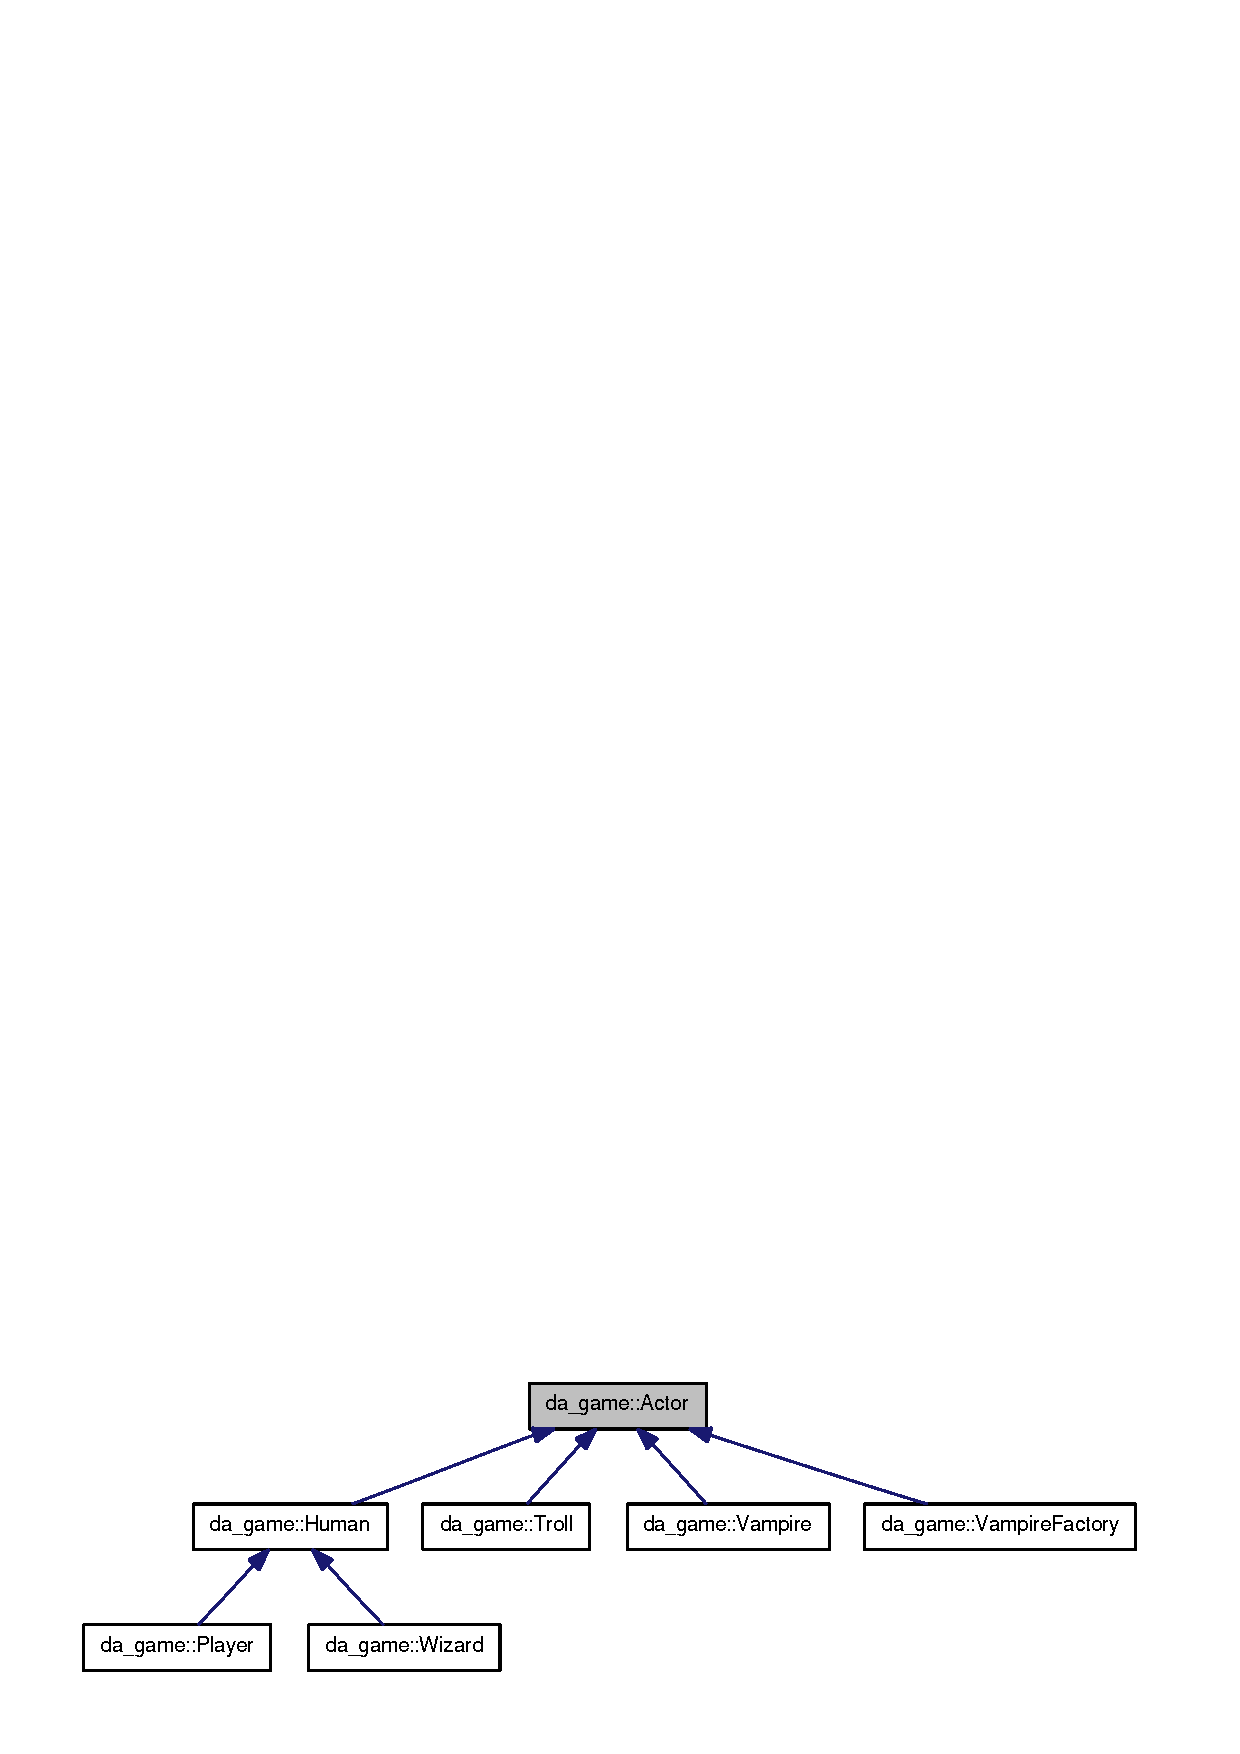
\includegraphics[width=400pt]{classda__game_1_1Actor__inherit__graph}
\end{center}
\end{figure}
Collaboration diagram for da\_\-game::Actor:\nopagebreak
\begin{figure}[H]
\begin{center}
\leavevmode
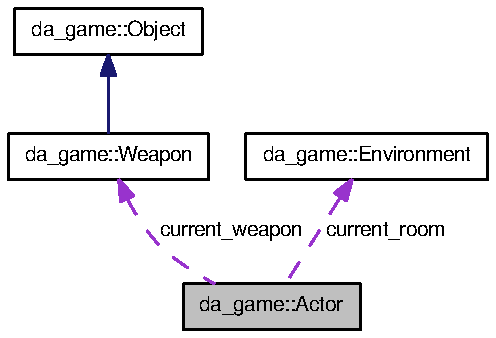
\includegraphics[width=274pt]{classda__game_1_1Actor__coll__graph}
\end{center}
\end{figure}
\subsection*{Public Member Functions}
\begin{DoxyCompactItemize}
\item 
\hypertarget{classda__game_1_1Actor_a4e1570c1f5ee72efaf2f17309e491d7e}{
virtual void {\bfseries run} ()=0}
\label{classda__game_1_1Actor_a4e1570c1f5ee72efaf2f17309e491d7e}

\item 
\hypertarget{classda__game_1_1Actor_adecbdf29f9cb31095b6b32fdf99dc72a}{
virtual std::string {\bfseries get\_\-type} () const =0}
\label{classda__game_1_1Actor_adecbdf29f9cb31095b6b32fdf99dc72a}

\item 
\hypertarget{classda__game_1_1Actor_a53656847acff24bc249e507d31909b86}{
virtual std::string {\bfseries get\_\-name} () const =0}
\label{classda__game_1_1Actor_a53656847acff24bc249e507d31909b86}

\item 
virtual void \hyperlink{classda__game_1_1Actor_a6be7923ecbacabf779eda60f1f78bb72}{go} (std::string)
\item 
\hypertarget{classda__game_1_1Actor_ac00094ad57edec1218e2c40008e8177a}{
virtual void {\bfseries pick\_\-up} (\hyperlink{classda__game_1_1Object}{Object} $\ast$)}
\label{classda__game_1_1Actor_ac00094ad57edec1218e2c40008e8177a}

\item 
\hypertarget{classda__game_1_1Actor_a412f9a1ef89acffa948e92434179143d}{
virtual bool {\bfseries drop} (\hyperlink{classda__game_1_1Object}{Object} $\ast$)}
\label{classda__game_1_1Actor_a412f9a1ef89acffa948e92434179143d}

\item 
\hypertarget{classda__game_1_1Actor_a4106856b26e95ba76708da5b0e497cc7}{
virtual void {\bfseries talk\_\-to} (\hyperlink{classda__game_1_1Actor}{Actor} \&)=0}
\label{classda__game_1_1Actor_a4106856b26e95ba76708da5b0e497cc7}

\item 
\hypertarget{classda__game_1_1Actor_ae7194d1dba4026c8333f9bc12041ce84}{
virtual \hyperlink{classda__game_1_1Weapon}{Weapon} $\ast$ {\bfseries weapon} ()}
\label{classda__game_1_1Actor_ae7194d1dba4026c8333f9bc12041ce84}

\item 
\hypertarget{classda__game_1_1Actor_a54f63c010e082f31dc3cbdbbfb7238e1}{
virtual void {\bfseries fight} (\hyperlink{classda__game_1_1Actor}{Actor} \&)}
\label{classda__game_1_1Actor_a54f63c010e082f31dc3cbdbbfb7238e1}

\end{DoxyCompactItemize}
\subsection*{Public Attributes}
\begin{DoxyCompactItemize}
\item 
\hypertarget{classda__game_1_1Actor_aa469aa0319da09f045ec836890fabf6a}{
const int {\bfseries id}}
\label{classda__game_1_1Actor_aa469aa0319da09f045ec836890fabf6a}

\end{DoxyCompactItemize}
\subsection*{Protected Attributes}
\begin{DoxyCompactItemize}
\item 
\hypertarget{classda__game_1_1Actor_ab5a5b98560a294c0feb2ccf5efb622ea}{
int {\bfseries hp}}
\label{classda__game_1_1Actor_ab5a5b98560a294c0feb2ccf5efb622ea}

\item 
\hypertarget{classda__game_1_1Actor_a134949b1c3dfe71dcadba6d6f9f0d13a}{
int {\bfseries strength}}
\label{classda__game_1_1Actor_a134949b1c3dfe71dcadba6d6f9f0d13a}

\item 
\hypertarget{classda__game_1_1Actor_ac5cc7b2e4c41e85f4222750065be7d80}{
\hyperlink{classda__game_1_1Weapon}{Weapon} $\ast$ {\bfseries current\_\-weapon}}
\label{classda__game_1_1Actor_ac5cc7b2e4c41e85f4222750065be7d80}

\item 
\hypertarget{classda__game_1_1Actor_a0c71533d0498330db5c211bc60147266}{
\hyperlink{classda__game_1_1Environment}{Environment} $\ast$ {\bfseries current\_\-room}}
\label{classda__game_1_1Actor_a0c71533d0498330db5c211bc60147266}

\item 
\hypertarget{classda__game_1_1Actor_ac01a6a22cde1b2e088cbddb81415e0b4}{
std::vector$<$ \hyperlink{classda__game_1_1Object}{Object} $\ast$ $>$ $\ast$ {\bfseries objects}}
\label{classda__game_1_1Actor_ac01a6a22cde1b2e088cbddb81415e0b4}

\end{DoxyCompactItemize}
\subsection*{Static Protected Attributes}
\begin{DoxyCompactItemize}
\item 
\hypertarget{classda__game_1_1Actor_a667364acb9cf6d06df598eeee2675212}{
static int {\bfseries instances}}
\label{classda__game_1_1Actor_a667364acb9cf6d06df598eeee2675212}

\end{DoxyCompactItemize}
\subsection*{Friends}
\begin{DoxyCompactItemize}
\item 
\hypertarget{classda__game_1_1Actor_ad58162d418e52e78ef2d13bea08472d4}{
class {\bfseries GameCommands}}
\label{classda__game_1_1Actor_ad58162d418e52e78ef2d13bea08472d4}

\end{DoxyCompactItemize}


\subsection{Member Function Documentation}
\hypertarget{classda__game_1_1Actor_a6be7923ecbacabf779eda60f1f78bb72}{
\index{da\_\-game::Actor@{da\_\-game::Actor}!go@{go}}
\index{go@{go}!da_game::Actor@{da\_\-game::Actor}}
\subsubsection[{go}]{\setlength{\rightskip}{0pt plus 5cm}void da\_\-game::Actor::go (std::string {\em exit\_\-name})\hspace{0.3cm}{\ttfamily  \mbox{[}virtual\mbox{]}}}}
\label{classda__game_1_1Actor_a6be7923ecbacabf779eda60f1f78bb72}
Takes this actor to the environment that the given exit leads to. However the exit must not be locked.


\begin{DoxyParams}{Parameters}
\item[{\em exit\_\-name}]The name of the exit to go through \end{DoxyParams}


Reimplemented in \hyperlink{classda__game_1_1VampireFactory_ab8f8fffebef4af1a90d00a0f011b245b}{da\_\-game::VampireFactory}.

The documentation for this class was generated from the following files:\begin{DoxyCompactItemize}
\item 
actor.h\item 
actor.cpp\end{DoxyCompactItemize}

\hypertarget{classda__game_1_1Bag}{
\section{da\_\-game::Bag Class Reference}
\label{classda__game_1_1Bag}\index{da\_\-game::Bag@{da\_\-game::Bag}}
}
Inheritance diagram for da\_\-game::Bag:\nopagebreak
\begin{figure}[H]
\begin{center}
\leavevmode
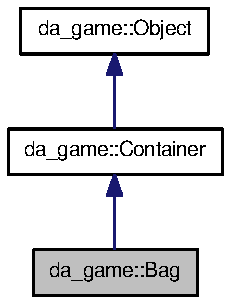
\includegraphics[width=146pt]{classda__game_1_1Bag__inherit__graph}
\end{center}
\end{figure}
Collaboration diagram for da\_\-game::Bag:\nopagebreak
\begin{figure}[H]
\begin{center}
\leavevmode
\includegraphics[width=146pt]{classda__game_1_1Bag__coll__graph}
\end{center}
\end{figure}
\subsection*{Public Member Functions}
\begin{DoxyCompactItemize}
\item 
\hypertarget{classda__game_1_1Bag_afb953efbb04ca4575bf0e1801174d10b}{
virtual int {\bfseries weight} () const }
\label{classda__game_1_1Bag_afb953efbb04ca4575bf0e1801174d10b}

\item 
\hypertarget{classda__game_1_1Bag_a40bb85eb64a085aa877ea9b6d12ab37c}{
virtual int {\bfseries volume} () const }
\label{classda__game_1_1Bag_a40bb85eb64a085aa877ea9b6d12ab37c}

\item 
\hypertarget{classda__game_1_1Bag_a92cbfb6c7526e991d7a85a6822ef8857}{
virtual int {\bfseries price} () const }
\label{classda__game_1_1Bag_a92cbfb6c7526e991d7a85a6822ef8857}

\item 
\hypertarget{classda__game_1_1Bag_a86ad15f7a2169cdc0971724460f18c14}{
virtual std::string {\bfseries type} () const }
\label{classda__game_1_1Bag_a86ad15f7a2169cdc0971724460f18c14}

\item 
\hypertarget{classda__game_1_1Bag_a697f83ee4ef9c2b8e4b79a38bfe03cfb}{
virtual int {\bfseries get\_\-hold\_\-weight} () const }
\label{classda__game_1_1Bag_a697f83ee4ef9c2b8e4b79a38bfe03cfb}

\item 
\hypertarget{classda__game_1_1Bag_ae4a79763c6ce34f702d93a245e12f806}{
virtual int {\bfseries get\_\-hold\_\-volume} () const }
\label{classda__game_1_1Bag_ae4a79763c6ce34f702d93a245e12f806}

\item 
\hypertarget{classda__game_1_1Bag_a9f64ac41fdaf87748e6684009cb83f3b}{
virtual bool {\bfseries add} (\hyperlink{classda__game_1_1Object}{Object} \&)}
\label{classda__game_1_1Bag_a9f64ac41fdaf87748e6684009cb83f3b}

\item 
\hypertarget{classda__game_1_1Bag_a91059470c55a1a89ffa5509397b6ef0f}{
virtual bool {\bfseries remove} (\hyperlink{classda__game_1_1Object}{Object} \&)}
\label{classda__game_1_1Bag_a91059470c55a1a89ffa5509397b6ef0f}

\end{DoxyCompactItemize}


The documentation for this class was generated from the following files:\begin{DoxyCompactItemize}
\item 
bag.h\item 
bag.cpp\end{DoxyCompactItemize}

\hypertarget{classda__game_1_1Container}{
\section{da\_\-game::Container Class Reference}
\label{classda__game_1_1Container}\index{da\_\-game::Container@{da\_\-game::Container}}
}
Inheritance diagram for da\_\-game::Container:\nopagebreak
\begin{figure}[H]
\begin{center}
\leavevmode
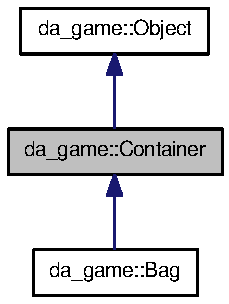
\includegraphics[width=146pt]{classda__game_1_1Container__inherit__graph}
\end{center}
\end{figure}
Collaboration diagram for da\_\-game::Container:\nopagebreak
\begin{figure}[H]
\begin{center}
\leavevmode
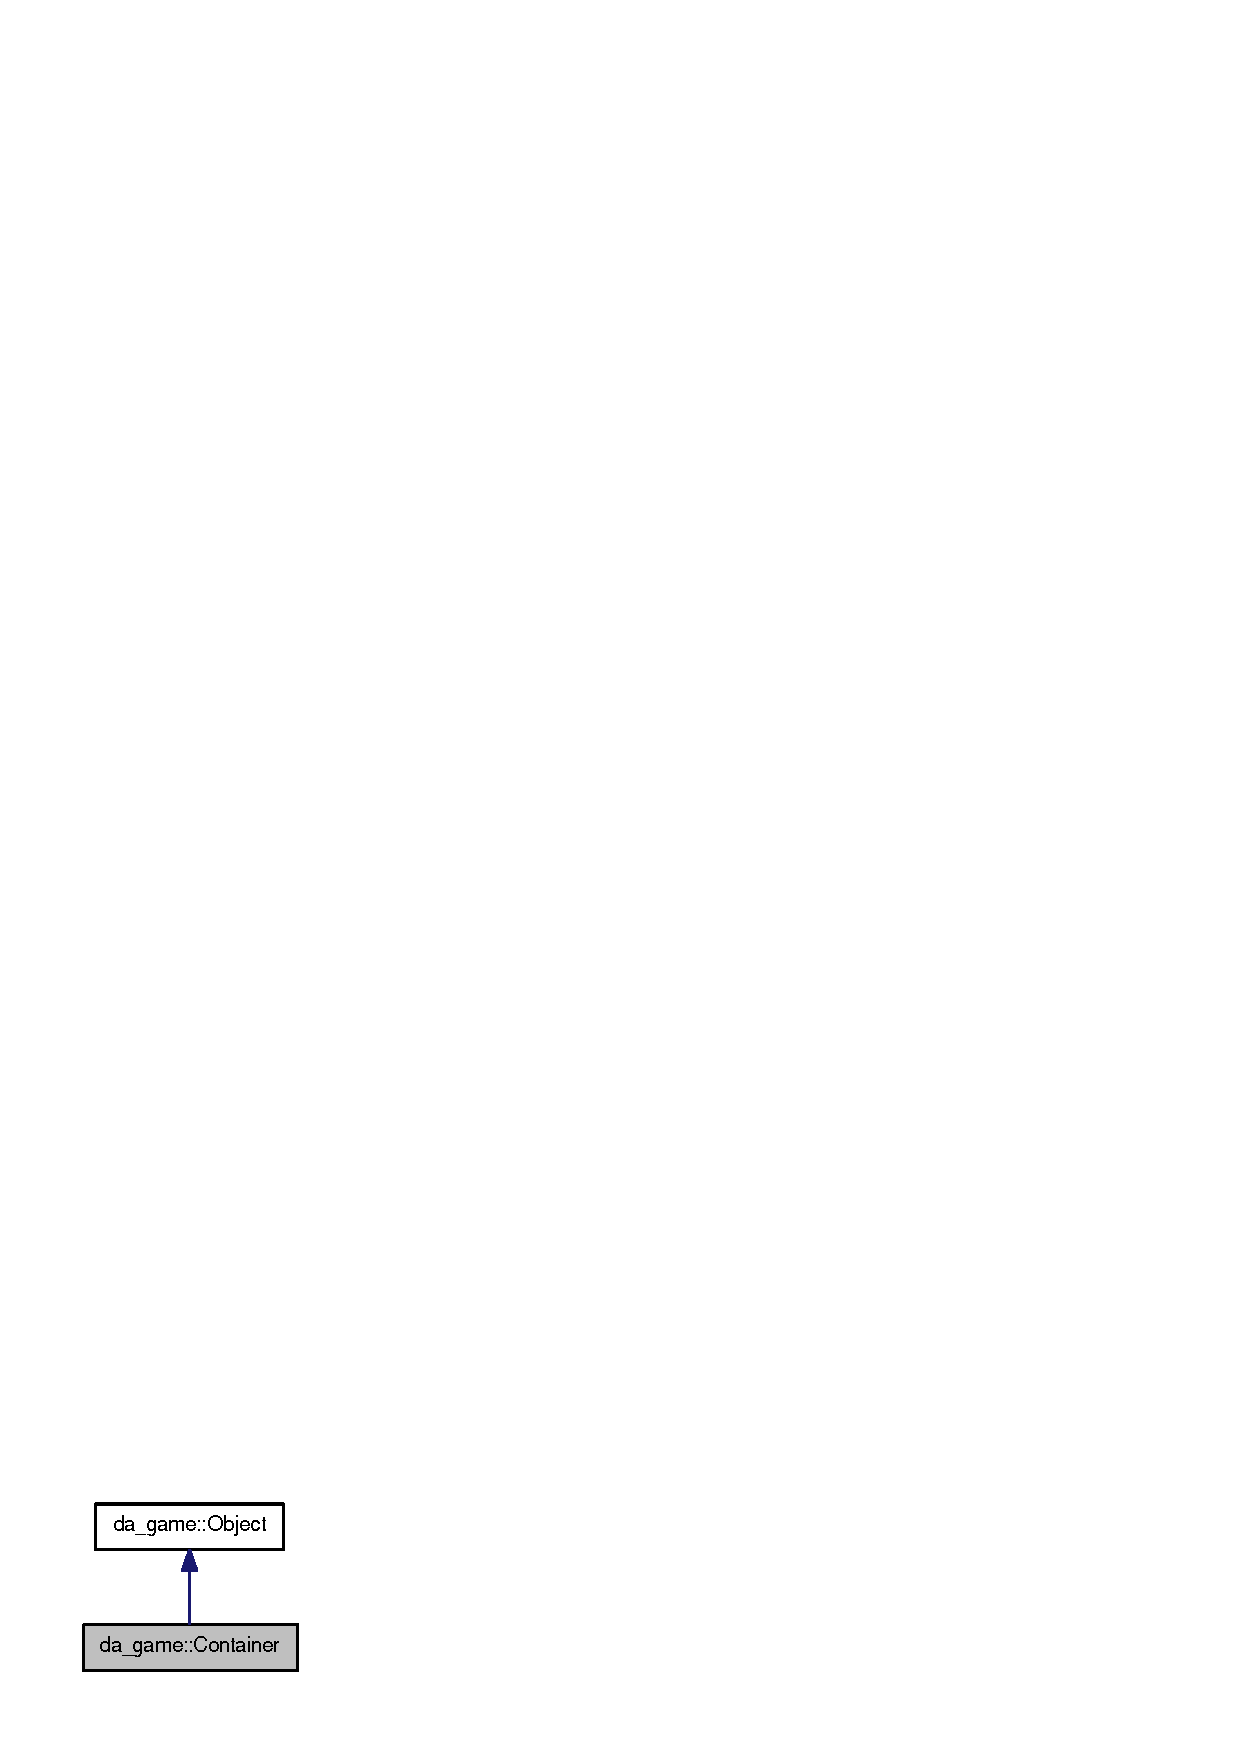
\includegraphics[width=146pt]{classda__game_1_1Container__coll__graph}
\end{center}
\end{figure}
\subsection*{Public Member Functions}
\begin{DoxyCompactItemize}
\item 
\hypertarget{classda__game_1_1Container_a8791f5bdac70b65d978ac0184ed48525}{
virtual int {\bfseries get\_\-hold\_\-weight} () const =0}
\label{classda__game_1_1Container_a8791f5bdac70b65d978ac0184ed48525}

\item 
\hypertarget{classda__game_1_1Container_a884311719474a432f186dfc803e15873}{
virtual int {\bfseries get\_\-hold\_\-volume} () const =0}
\label{classda__game_1_1Container_a884311719474a432f186dfc803e15873}

\item 
\hypertarget{classda__game_1_1Container_a32807c145257173e5bb2948c8a7d5207}{
virtual int {\bfseries get\_\-weight\_\-left} () const }
\label{classda__game_1_1Container_a32807c145257173e5bb2948c8a7d5207}

\item 
\hypertarget{classda__game_1_1Container_a1fb472908ed21d8268caa65374e195b4}{
virtual int {\bfseries get\_\-volume\_\-left} () const }
\label{classda__game_1_1Container_a1fb472908ed21d8268caa65374e195b4}

\item 
\hypertarget{classda__game_1_1Container_a37fab4911cc993db3f4e26c4e6e95eba}{
virtual bool {\bfseries add} (\hyperlink{classda__game_1_1Object}{Object} \&)=0}
\label{classda__game_1_1Container_a37fab4911cc993db3f4e26c4e6e95eba}

\item 
\hypertarget{classda__game_1_1Container_a8bb5c906abd5f6df854e6eab8831305e}{
virtual bool {\bfseries remove} (\hyperlink{classda__game_1_1Object}{Object} \&)=0}
\label{classda__game_1_1Container_a8bb5c906abd5f6df854e6eab8831305e}

\item 
\hypertarget{classda__game_1_1Container_a77eaf77a8ae8f4ddc16067102379f357}{
virtual std::vector$<$ \hyperlink{classda__game_1_1Object}{Object} $\ast$ $>$ $\ast$ {\bfseries get\_\-objects} ()}
\label{classda__game_1_1Container_a77eaf77a8ae8f4ddc16067102379f357}

\end{DoxyCompactItemize}
\subsection*{Protected Attributes}
\begin{DoxyCompactItemize}
\item 
\hypertarget{classda__game_1_1Container_ae00fef93faf3dd5a8535845d0e7f63a0}{
int {\bfseries hold\_\-weight}}
\label{classda__game_1_1Container_ae00fef93faf3dd5a8535845d0e7f63a0}

\item 
\hypertarget{classda__game_1_1Container_aae21247d0254a4e272065b6141795514}{
int {\bfseries hold\_\-volume}}
\label{classda__game_1_1Container_aae21247d0254a4e272065b6141795514}

\item 
\hypertarget{classda__game_1_1Container_ac06cad31bb04667d3fb88c2311422373}{
std::vector$<$ \hyperlink{classda__game_1_1Object}{Object} $\ast$ $>$ $\ast$ {\bfseries objects}}
\label{classda__game_1_1Container_ac06cad31bb04667d3fb88c2311422373}

\end{DoxyCompactItemize}


The documentation for this class was generated from the following files:\begin{DoxyCompactItemize}
\item 
container.h\item 
container.cpp\end{DoxyCompactItemize}

\hypertarget{classda__game_1_1DefaultWeapon}{
\section{da\_\-game::DefaultWeapon Class Reference}
\label{classda__game_1_1DefaultWeapon}\index{da\_\-game::DefaultWeapon@{da\_\-game::DefaultWeapon}}
}
Inheritance diagram for da\_\-game::DefaultWeapon:\nopagebreak
\begin{figure}[H]
\begin{center}
\leavevmode
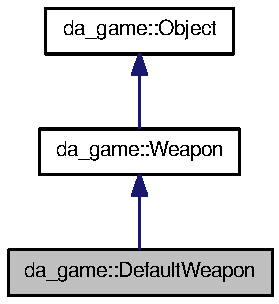
\includegraphics[width=170pt]{classda__game_1_1DefaultWeapon__inherit__graph}
\end{center}
\end{figure}
Collaboration diagram for da\_\-game::DefaultWeapon:\nopagebreak
\begin{figure}[H]
\begin{center}
\leavevmode
\includegraphics[width=170pt]{classda__game_1_1DefaultWeapon__coll__graph}
\end{center}
\end{figure}
\subsection*{Public Member Functions}
\begin{DoxyCompactItemize}
\item 
\hypertarget{classda__game_1_1DefaultWeapon_aa827b7dd05281ad20ff869666e493f5d}{
int {\bfseries weight} () const }
\label{classda__game_1_1DefaultWeapon_aa827b7dd05281ad20ff869666e493f5d}

\item 
\hypertarget{classda__game_1_1DefaultWeapon_a446988bb259fb96132fd7fb24da798f0}{
int {\bfseries volume} () const }
\label{classda__game_1_1DefaultWeapon_a446988bb259fb96132fd7fb24da798f0}

\item 
\hypertarget{classda__game_1_1DefaultWeapon_ac6c71d1c8cda696dc372a0e436dfcc98}{
int {\bfseries price} () const }
\label{classda__game_1_1DefaultWeapon_ac6c71d1c8cda696dc372a0e436dfcc98}

\end{DoxyCompactItemize}


The documentation for this class was generated from the following files:\begin{DoxyCompactItemize}
\item 
default\_\-weapon.h\item 
default\_\-weapon.cpp\end{DoxyCompactItemize}

\hypertarget{classda__game_1_1Environment}{
\section{da\_\-game::Environment Class Reference}
\label{classda__game_1_1Environment}\index{da\_\-game::Environment@{da\_\-game::Environment}}
}
Inheritance diagram for da\_\-game::Environment::\begin{figure}[H]
\begin{center}
\leavevmode
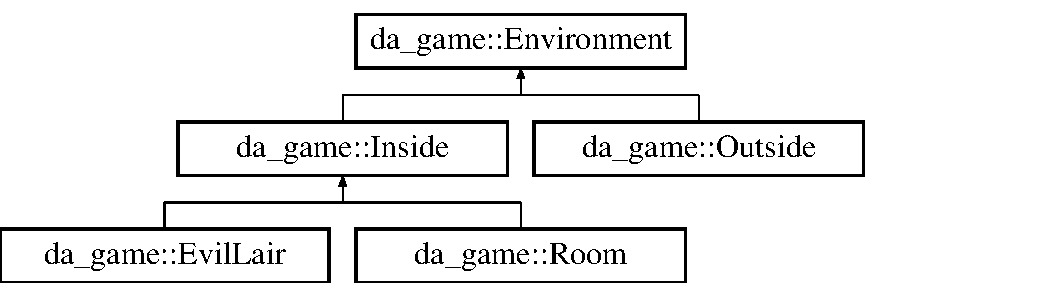
\includegraphics[height=3cm]{classda__game_1_1Environment}
\end{center}
\end{figure}
\subsection*{Public Member Functions}
\begin{DoxyCompactItemize}
\item 
\hypertarget{classda__game_1_1Environment_a412ec5b8713e11bbee66dde20076ed2f}{
virtual std::string {\bfseries description} () const }
\label{classda__game_1_1Environment_a412ec5b8713e11bbee66dde20076ed2f}

\item 
virtual bool \hyperlink{classda__game_1_1Environment_a7b8062cb2c63bb225225a9749da4e8cf}{add\_\-exit} (std::string, \hyperlink{classda__game_1_1Exit}{Exit} $\ast$)
\item 
virtual \hyperlink{classda__game_1_1Exit}{Exit} $\ast$ \hyperlink{classda__game_1_1Environment_ad0b26526cf4a76fa7827ab6cb539d98b}{get\_\-exit} (std::string) const 
\item 
virtual std::vector$<$ std::string $>$ \hyperlink{classda__game_1_1Environment_a1702d13f246e537540f1073a138a706d}{get\_\-exit\_\-names} () const 
\item 
virtual void \hyperlink{classda__game_1_1Environment_a194d9cfcdf2c86431d83dd5bc686c489}{enter} (\hyperlink{classda__game_1_1Actor}{Actor} \&)
\item 
virtual void \hyperlink{classda__game_1_1Environment_aed5b6d00da5afb0dae96bedcb9ee9642}{leave} (\hyperlink{classda__game_1_1Actor}{Actor} \&)
\item 
virtual bool \hyperlink{classda__game_1_1Environment_a1160cb0cffc0f37e058f58457c76d12b}{pick\_\-up} (\hyperlink{classda__game_1_1Object}{Object} $\ast$)
\item 
virtual void \hyperlink{classda__game_1_1Environment_a4d1fb3198721b013f77b79cea398bd35}{drop} (\hyperlink{classda__game_1_1Object}{Object} $\ast$)
\item 
\hypertarget{classda__game_1_1Environment_aa961ca9cba24dd62107ddcb5c5b5ab29}{
virtual std::vector$<$ \hyperlink{classda__game_1_1Object}{Object} $\ast$ $>$ {\bfseries get\_\-objects} ()}
\label{classda__game_1_1Environment_aa961ca9cba24dd62107ddcb5c5b5ab29}

\item 
\hypertarget{classda__game_1_1Environment_ad5248ea56c5bf7038ae48d7326d361f4}{
virtual std::vector$<$ \hyperlink{classda__game_1_1Actor}{Actor} $\ast$ $>$ {\bfseries get\_\-actors} ()}
\label{classda__game_1_1Environment_ad5248ea56c5bf7038ae48d7326d361f4}

\end{DoxyCompactItemize}
\subsection*{Protected Attributes}
\begin{DoxyCompactItemize}
\item 
\hypertarget{classda__game_1_1Environment_afd10beaae82f22e4ea970b9a85b1f57c}{
std::vector$<$ \hyperlink{classda__game_1_1Object}{Object} $\ast$ $>$ $\ast$ {\bfseries objects}}
\label{classda__game_1_1Environment_afd10beaae82f22e4ea970b9a85b1f57c}

\item 
\hypertarget{classda__game_1_1Environment_a2d4baf7e9c6a619ef692edb0287f5df7}{
std::vector$<$ \hyperlink{classda__game_1_1Actor}{Actor} $\ast$ $>$ $\ast$ {\bfseries actors}}
\label{classda__game_1_1Environment_a2d4baf7e9c6a619ef692edb0287f5df7}

\item 
\hypertarget{classda__game_1_1Environment_a40544e6d69042fc864b1c8057ad0bc16}{
std::map$<$ std::string, \hyperlink{classda__game_1_1Environment}{Environment} $\ast$ $>$ {\bfseries neighbors}}
\label{classda__game_1_1Environment_a40544e6d69042fc864b1c8057ad0bc16}

\item 
\hypertarget{classda__game_1_1Environment_a332747dd172e39880f0703283e5fcf23}{
std::map$<$ std::string, \hyperlink{classda__game_1_1Exit}{Exit} $\ast$ $>$ {\bfseries exits}}
\label{classda__game_1_1Environment_a332747dd172e39880f0703283e5fcf23}

\end{DoxyCompactItemize}
\subsection*{Friends}
\begin{DoxyCompactItemize}
\item 
\hypertarget{classda__game_1_1Environment_ad58162d418e52e78ef2d13bea08472d4}{
class {\bfseries GameCommands}}
\label{classda__game_1_1Environment_ad58162d418e52e78ef2d13bea08472d4}

\end{DoxyCompactItemize}


\subsection{Member Function Documentation}
\hypertarget{classda__game_1_1Environment_a7b8062cb2c63bb225225a9749da4e8cf}{
\index{da\_\-game::Environment@{da\_\-game::Environment}!add\_\-exit@{add\_\-exit}}
\index{add\_\-exit@{add\_\-exit}!da_game::Environment@{da\_\-game::Environment}}
\subsubsection[{add\_\-exit}]{\setlength{\rightskip}{0pt plus 5cm}bool da\_\-game::Environment::add\_\-exit (std::string {\em name}, \/  {\bf Exit} $\ast$ {\em exit})\hspace{0.3cm}{\ttfamily  \mbox{[}virtual\mbox{]}}}}
\label{classda__game_1_1Environment_a7b8062cb2c63bb225225a9749da4e8cf}
Adds the specified exit with the given name (preferably a point of the compass) to this environment.

\begin{DoxyReturn}{Returns}
True if the exit was added or false if an exit with the same value already existed 
\end{DoxyReturn}
\hypertarget{classda__game_1_1Environment_a4d1fb3198721b013f77b79cea398bd35}{
\index{da\_\-game::Environment@{da\_\-game::Environment}!drop@{drop}}
\index{drop@{drop}!da_game::Environment@{da\_\-game::Environment}}
\subsubsection[{drop}]{\setlength{\rightskip}{0pt plus 5cm}void da\_\-game::Environment::drop ({\bf Object} $\ast$ {\em object})\hspace{0.3cm}{\ttfamily  \mbox{[}virtual\mbox{]}}}}
\label{classda__game_1_1Environment_a4d1fb3198721b013f77b79cea398bd35}
Someone drops an object in this environment. That means this environment must take care of it.


\begin{DoxyParams}{Parameters}
\item[{\em object}]The object that is being dropped \end{DoxyParams}
\hypertarget{classda__game_1_1Environment_a194d9cfcdf2c86431d83dd5bc686c489}{
\index{da\_\-game::Environment@{da\_\-game::Environment}!enter@{enter}}
\index{enter@{enter}!da_game::Environment@{da\_\-game::Environment}}
\subsubsection[{enter}]{\setlength{\rightskip}{0pt plus 5cm}void da\_\-game::Environment::enter ({\bf Actor} \& {\em actor})\hspace{0.3cm}{\ttfamily  \mbox{[}virtual\mbox{]}}}}
\label{classda__game_1_1Environment_a194d9cfcdf2c86431d83dd5bc686c489}
Lets the specified actor enter this environment.


\begin{DoxyParams}{Parameters}
\item[{\em actor}]The actor to enter \end{DoxyParams}
\hypertarget{classda__game_1_1Environment_ad0b26526cf4a76fa7827ab6cb539d98b}{
\index{da\_\-game::Environment@{da\_\-game::Environment}!get\_\-exit@{get\_\-exit}}
\index{get\_\-exit@{get\_\-exit}!da_game::Environment@{da\_\-game::Environment}}
\subsubsection[{get\_\-exit}]{\setlength{\rightskip}{0pt plus 5cm}{\bf Exit} $\ast$ da\_\-game::Environment::get\_\-exit (std::string {\em name}) const\hspace{0.3cm}{\ttfamily  \mbox{[}virtual\mbox{]}}}}
\label{classda__game_1_1Environment_ad0b26526cf4a76fa7827ab6cb539d98b}
Returns the exit with the given name, if there is a such.


\begin{DoxyParams}{Parameters}
\item[{\em name}]The name of the exit \end{DoxyParams}
\begin{DoxyReturn}{Returns}
The exit with the given name 
\end{DoxyReturn}
\hypertarget{classda__game_1_1Environment_a1702d13f246e537540f1073a138a706d}{
\index{da\_\-game::Environment@{da\_\-game::Environment}!get\_\-exit\_\-names@{get\_\-exit\_\-names}}
\index{get\_\-exit\_\-names@{get\_\-exit\_\-names}!da_game::Environment@{da\_\-game::Environment}}
\subsubsection[{get\_\-exit\_\-names}]{\setlength{\rightskip}{0pt plus 5cm}std::vector$<$ std::string $>$ da\_\-game::Environment::get\_\-exit\_\-names () const\hspace{0.3cm}{\ttfamily  \mbox{[}virtual\mbox{]}}}}
\label{classda__game_1_1Environment_a1702d13f246e537540f1073a138a706d}
Returns a list of all available exits in this environment.

\begin{DoxyReturn}{Returns}
List of exits 
\end{DoxyReturn}
\hypertarget{classda__game_1_1Environment_aed5b6d00da5afb0dae96bedcb9ee9642}{
\index{da\_\-game::Environment@{da\_\-game::Environment}!leave@{leave}}
\index{leave@{leave}!da_game::Environment@{da\_\-game::Environment}}
\subsubsection[{leave}]{\setlength{\rightskip}{0pt plus 5cm}void da\_\-game::Environment::leave ({\bf Actor} \& {\em actor})\hspace{0.3cm}{\ttfamily  \mbox{[}virtual\mbox{]}}}}
\label{classda__game_1_1Environment_aed5b6d00da5afb0dae96bedcb9ee9642}
Lets an actor leave this environment.


\begin{DoxyParams}{Parameters}
\item[{\em actor}]The actor to leave \end{DoxyParams}
\hypertarget{classda__game_1_1Environment_a1160cb0cffc0f37e058f58457c76d12b}{
\index{da\_\-game::Environment@{da\_\-game::Environment}!pick\_\-up@{pick\_\-up}}
\index{pick\_\-up@{pick\_\-up}!da_game::Environment@{da\_\-game::Environment}}
\subsubsection[{pick\_\-up}]{\setlength{\rightskip}{0pt plus 5cm}bool da\_\-game::Environment::pick\_\-up ({\bf Object} $\ast$ {\em object})\hspace{0.3cm}{\ttfamily  \mbox{[}virtual\mbox{]}}}}
\label{classda__game_1_1Environment_a1160cb0cffc0f37e058f58457c76d12b}
Someone picks up an object that is owned by this environment. That means this environment must hand over the object in question.


\begin{DoxyParams}{Parameters}
\item[{\em object}]The object that is being picked up \end{DoxyParams}
\begin{DoxyReturn}{Returns}
True if the object really was held by this environment, otherwise false. 
\end{DoxyReturn}


The documentation for this class was generated from the following files:\begin{DoxyCompactItemize}
\item 
environment.h\item 
actor.cpp\item 
environment.cpp\end{DoxyCompactItemize}

\hypertarget{classda__game_1_1EvilLair}{
\section{da\_\-game::EvilLair Class Reference}
\label{classda__game_1_1EvilLair}\index{da\_\-game::EvilLair@{da\_\-game::EvilLair}}
}
Inheritance diagram for da\_\-game::EvilLair::\begin{figure}[H]
\begin{center}
\leavevmode
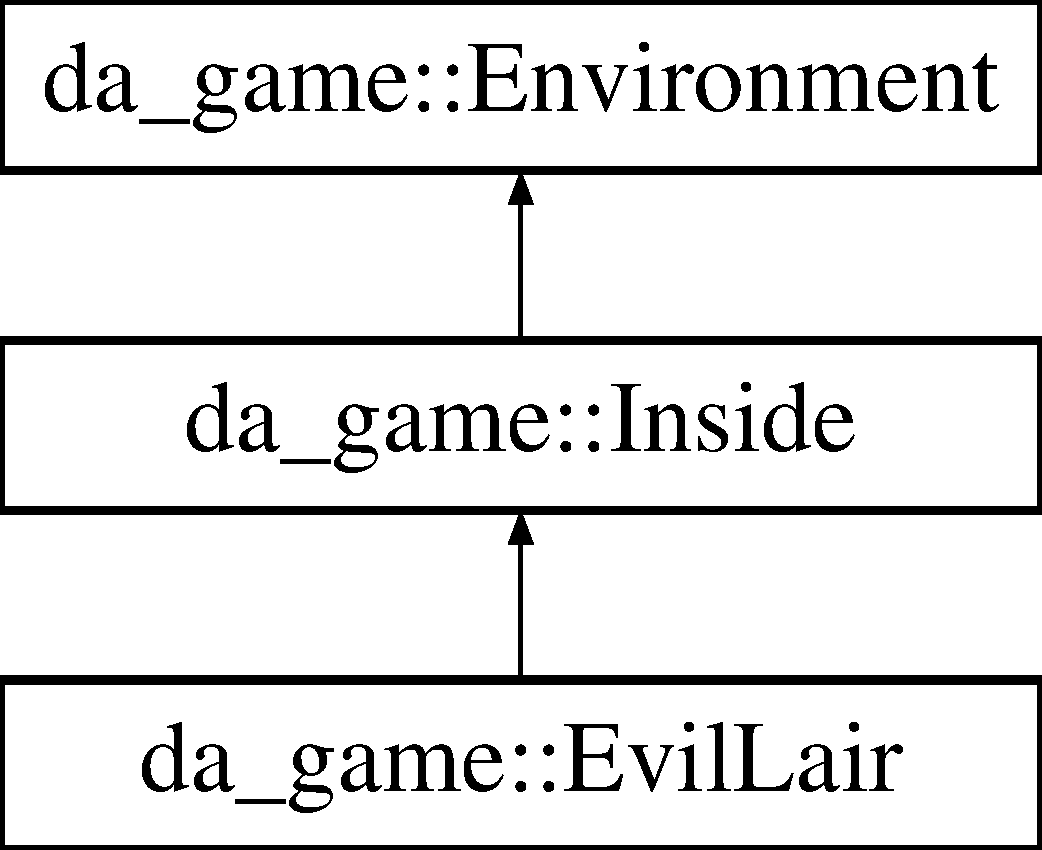
\includegraphics[height=3cm]{classda__game_1_1EvilLair}
\end{center}
\end{figure}
\subsection*{Public Member Functions}
\begin{DoxyCompactItemize}
\item 
\hyperlink{classda__game_1_1EvilLair_afe4fe8ac046b4c91ad4e0a0fd4ba7baf}{EvilLair} ()
\item 
\hypertarget{classda__game_1_1EvilLair_adb5a496c651f24ed91e8fdf51c821787}{
virtual std::string {\bfseries description} () const }
\label{classda__game_1_1EvilLair_adb5a496c651f24ed91e8fdf51c821787}

\end{DoxyCompactItemize}


\subsection{Constructor \& Destructor Documentation}
\hypertarget{classda__game_1_1EvilLair_afe4fe8ac046b4c91ad4e0a0fd4ba7baf}{
\index{da\_\-game::EvilLair@{da\_\-game::EvilLair}!EvilLair@{EvilLair}}
\index{EvilLair@{EvilLair}!da_game::EvilLair@{da\_\-game::EvilLair}}
\subsubsection[{EvilLair}]{\setlength{\rightskip}{0pt plus 5cm}da\_\-game::EvilLair::EvilLair ()}}
\label{classda__game_1_1EvilLair_afe4fe8ac046b4c91ad4e0a0fd4ba7baf}
Constructs an empty evil lair 

The documentation for this class was generated from the following files:\begin{DoxyCompactItemize}
\item 
evil\_\-lair.h\item 
evil\_\-lair.cpp\end{DoxyCompactItemize}

\hypertarget{classda__game_1_1Exit}{
\section{da\_\-game::Exit Class Reference}
\label{classda__game_1_1Exit}\index{da\_\-game::Exit@{da\_\-game::Exit}}
}


{\ttfamily \#include $<$exit.h$>$}\subsection*{Public Member Functions}
\begin{DoxyCompactItemize}
\item 
\hyperlink{classda__game_1_1Exit_aaacef438c545390f01c5bf1c6072d43e}{Exit} ()
\item 
\hyperlink{classda__game_1_1Exit_ae6a2d9ab456888b9c5aa7e23539b2827}{Exit} (\hyperlink{classda__game_1_1Environment}{Environment} $\ast$, bool has\_\-lock=false, std::string code=\char`\"{}\char`\"{}, bool locked=false, std::string desc=\char`\"{}\char`\"{})
\item 
\hyperlink{classda__game_1_1Environment}{Environment} $\ast$ \hyperlink{classda__game_1_1Exit_ad4f4951039d5d7ca57fce2120e8390f4}{get\_\-outfall} () const 
\item 
bool \hyperlink{classda__game_1_1Exit_a469187cf61ab5285b71ac4fb103f10b1}{is\_\-locked} ()
\item 
void \hyperlink{classda__game_1_1Exit_ae4f9caa0ac7bf7e09ae1b32fd3f10719}{set\_\-outfall} (\hyperlink{classda__game_1_1Environment}{Environment} $\ast$)
\item 
void \hyperlink{classda__game_1_1Exit_aef620aed29423172be98f0e2bc12db13}{set\_\-description} (std::string)
\item 
void \hyperlink{classda__game_1_1Exit_ad79677f119a5d06a6d4a9185c710ab73}{set\_\-key\_\-code} (std::string)
\item 
void \hyperlink{classda__game_1_1Exit_a48bfb84dc93e05cb9f43d9d87726b8f5}{set\_\-locked} (bool)
\item 
bool \hyperlink{classda__game_1_1Exit_a252eecd61a98bec46db93185745deff5}{lock} (\hyperlink{classda__game_1_1Key}{Key} $\ast$)
\item 
bool \hyperlink{classda__game_1_1Exit_a4e770f624717bb87b2ebd372eb71a09c}{unlock} (\hyperlink{classda__game_1_1Key}{Key} $\ast$)
\item 
bool \hyperlink{classda__game_1_1Exit_a36b7a9235fcb00bf2be0b3fbc5817310}{toggle\_\-lock} (\hyperlink{classda__game_1_1Key}{Key} $\ast$)
\end{DoxyCompactItemize}


\subsection{Detailed Description}
Exits are used in environments to allow actors travelling between different environments. 

\subsection{Constructor \& Destructor Documentation}
\hypertarget{classda__game_1_1Exit_aaacef438c545390f01c5bf1c6072d43e}{
\index{da\_\-game::Exit@{da\_\-game::Exit}!Exit@{Exit}}
\index{Exit@{Exit}!da_game::Exit@{da\_\-game::Exit}}
\subsubsection[{Exit}]{\setlength{\rightskip}{0pt plus 5cm}da\_\-game::Exit::Exit ()}}
\label{classda__game_1_1Exit_aaacef438c545390f01c5bf1c6072d43e}
Creates a new exit with some default parameters, but without any outfall. This is probably useless unless an outfall is later set. \hypertarget{classda__game_1_1Exit_ae6a2d9ab456888b9c5aa7e23539b2827}{
\index{da\_\-game::Exit@{da\_\-game::Exit}!Exit@{Exit}}
\index{Exit@{Exit}!da_game::Exit@{da\_\-game::Exit}}
\subsubsection[{Exit}]{\setlength{\rightskip}{0pt plus 5cm}da\_\-game::Exit::Exit ({\bf Environment} $\ast$ {\em outfall}, \/  bool {\em has\_\-lock} = {\ttfamily false}, \/  std::string {\em key\_\-code} = {\ttfamily \char`\"{}\char`\"{}}, \/  bool {\em locked} = {\ttfamily false}, \/  std::string {\em description} = {\ttfamily \char`\"{}\char`\"{}})\hspace{0.3cm}{\ttfamily  \mbox{[}explicit\mbox{]}}}}
\label{classda__game_1_1Exit_ae6a2d9ab456888b9c5aa7e23539b2827}
Constructs a new exit with the given outfall and description.

Notice: All parameters except outfall are given default values if not specified.


\begin{DoxyParams}{Parameters}
\item[{\em outfall}]Where this exit leads to \item[{\em has\_\-lock}]Whether or not this exit has a lock \item[{\em key\_\-code}]The key code for this exit \item[{\em locked}]The locked state of this exit \item[{\em description}]A short description of this exit \end{DoxyParams}


\subsection{Member Function Documentation}
\hypertarget{classda__game_1_1Exit_ad4f4951039d5d7ca57fce2120e8390f4}{
\index{da\_\-game::Exit@{da\_\-game::Exit}!get\_\-outfall@{get\_\-outfall}}
\index{get\_\-outfall@{get\_\-outfall}!da_game::Exit@{da\_\-game::Exit}}
\subsubsection[{get\_\-outfall}]{\setlength{\rightskip}{0pt plus 5cm}{\bf Environment} $\ast$ da\_\-game::Exit::get\_\-outfall () const}}
\label{classda__game_1_1Exit_ad4f4951039d5d7ca57fce2120e8390f4}
Returns the outfall of this exit, that is, where it leads to.

\begin{DoxyReturn}{Returns}
The outfall 
\end{DoxyReturn}
\hypertarget{classda__game_1_1Exit_a469187cf61ab5285b71ac4fb103f10b1}{
\index{da\_\-game::Exit@{da\_\-game::Exit}!is\_\-locked@{is\_\-locked}}
\index{is\_\-locked@{is\_\-locked}!da_game::Exit@{da\_\-game::Exit}}
\subsubsection[{is\_\-locked}]{\setlength{\rightskip}{0pt plus 5cm}bool da\_\-game::Exit::is\_\-locked ()}}
\label{classda__game_1_1Exit_a469187cf61ab5285b71ac4fb103f10b1}
Returns whether or not this exit is locked.

\begin{DoxyReturn}{Returns}
true if locked, false otherwise 
\end{DoxyReturn}
\hypertarget{classda__game_1_1Exit_a252eecd61a98bec46db93185745deff5}{
\index{da\_\-game::Exit@{da\_\-game::Exit}!lock@{lock}}
\index{lock@{lock}!da_game::Exit@{da\_\-game::Exit}}
\subsubsection[{lock}]{\setlength{\rightskip}{0pt plus 5cm}bool da\_\-game::Exit::lock ({\bf Key} $\ast$ {\em key})}}
\label{classda__game_1_1Exit_a252eecd61a98bec46db93185745deff5}
Locks this exit iff it has a lock and the key code from the specified key agrees to the one of this exit.


\begin{DoxyParams}{Parameters}
\item[{\em key}]The key to lock with \end{DoxyParams}
\begin{DoxyReturn}{Returns}
The new locked state of this exit 
\end{DoxyReturn}
\hypertarget{classda__game_1_1Exit_aef620aed29423172be98f0e2bc12db13}{
\index{da\_\-game::Exit@{da\_\-game::Exit}!set\_\-description@{set\_\-description}}
\index{set\_\-description@{set\_\-description}!da_game::Exit@{da\_\-game::Exit}}
\subsubsection[{set\_\-description}]{\setlength{\rightskip}{0pt plus 5cm}void da\_\-game::Exit::set\_\-description (std::string {\em description})}}
\label{classda__game_1_1Exit_aef620aed29423172be98f0e2bc12db13}
Sets the description of this exit to the one specified.


\begin{DoxyParams}{Parameters}
\item[{\em description}]The new description \end{DoxyParams}
\hypertarget{classda__game_1_1Exit_ad79677f119a5d06a6d4a9185c710ab73}{
\index{da\_\-game::Exit@{da\_\-game::Exit}!set\_\-key\_\-code@{set\_\-key\_\-code}}
\index{set\_\-key\_\-code@{set\_\-key\_\-code}!da_game::Exit@{da\_\-game::Exit}}
\subsubsection[{set\_\-key\_\-code}]{\setlength{\rightskip}{0pt plus 5cm}void da\_\-game::Exit::set\_\-key\_\-code (std::string {\em key\_\-code})}}
\label{classda__game_1_1Exit_ad79677f119a5d06a6d4a9185c710ab73}
Sets this exit's key code that is required in order to unlock it.


\begin{DoxyParams}{Parameters}
\item[{\em key\_\-code}]The new key code \end{DoxyParams}
\hypertarget{classda__game_1_1Exit_a48bfb84dc93e05cb9f43d9d87726b8f5}{
\index{da\_\-game::Exit@{da\_\-game::Exit}!set\_\-locked@{set\_\-locked}}
\index{set\_\-locked@{set\_\-locked}!da_game::Exit@{da\_\-game::Exit}}
\subsubsection[{set\_\-locked}]{\setlength{\rightskip}{0pt plus 5cm}void da\_\-game::Exit::set\_\-locked (bool {\em locked})}}
\label{classda__game_1_1Exit_a48bfb84dc93e05cb9f43d9d87726b8f5}
Sets the locked state of this exit.


\begin{DoxyParams}{Parameters}
\item[{\em locked}]Whether or not this exit is locked \end{DoxyParams}
\hypertarget{classda__game_1_1Exit_ae4f9caa0ac7bf7e09ae1b32fd3f10719}{
\index{da\_\-game::Exit@{da\_\-game::Exit}!set\_\-outfall@{set\_\-outfall}}
\index{set\_\-outfall@{set\_\-outfall}!da_game::Exit@{da\_\-game::Exit}}
\subsubsection[{set\_\-outfall}]{\setlength{\rightskip}{0pt plus 5cm}void da\_\-game::Exit::set\_\-outfall ({\bf Environment} $\ast$ {\em outfall})}}
\label{classda__game_1_1Exit_ae4f9caa0ac7bf7e09ae1b32fd3f10719}
Sets what environment this exit leads to.


\begin{DoxyParams}{Parameters}
\item[{\em outfall}]The new environment this exit should lead to \end{DoxyParams}
\hypertarget{classda__game_1_1Exit_a36b7a9235fcb00bf2be0b3fbc5817310}{
\index{da\_\-game::Exit@{da\_\-game::Exit}!toggle\_\-lock@{toggle\_\-lock}}
\index{toggle\_\-lock@{toggle\_\-lock}!da_game::Exit@{da\_\-game::Exit}}
\subsubsection[{toggle\_\-lock}]{\setlength{\rightskip}{0pt plus 5cm}bool da\_\-game::Exit::toggle\_\-lock ({\bf Key} $\ast$ {\em key})}}
\label{classda__game_1_1Exit_a36b7a9235fcb00bf2be0b3fbc5817310}
Toggles the status of this exit's lock; if it is locked it gets unlocked and vice versa. However, this does only work if the correct key is provided.


\begin{DoxyParams}{Parameters}
\item[{\em key}]The key to lock/unlock with \end{DoxyParams}
\begin{DoxyReturn}{Returns}
The new locked status of this exit 
\end{DoxyReturn}
\hypertarget{classda__game_1_1Exit_a4e770f624717bb87b2ebd372eb71a09c}{
\index{da\_\-game::Exit@{da\_\-game::Exit}!unlock@{unlock}}
\index{unlock@{unlock}!da_game::Exit@{da\_\-game::Exit}}
\subsubsection[{unlock}]{\setlength{\rightskip}{0pt plus 5cm}bool da\_\-game::Exit::unlock ({\bf Key} $\ast$ {\em key})}}
\label{classda__game_1_1Exit_a4e770f624717bb87b2ebd372eb71a09c}
Unlocks this exit iff this exit has a lock and the key code of the specified key equals the one of this exit.


\begin{DoxyParams}{Parameters}
\item[{\em key}]The key to unlock with \end{DoxyParams}
\begin{DoxyReturn}{Returns}
The new locked state of this exit 
\end{DoxyReturn}


The documentation for this class was generated from the following files:\begin{DoxyCompactItemize}
\item 
exit.h\item 
exit.cpp\end{DoxyCompactItemize}

\hypertarget{classda__game_1_1Food}{
\section{da\_\-game::Food Class Reference}
\label{classda__game_1_1Food}\index{da\_\-game::Food@{da\_\-game::Food}}
}
Inheritance diagram for da\_\-game::Food::\begin{figure}[H]
\begin{center}
\leavevmode
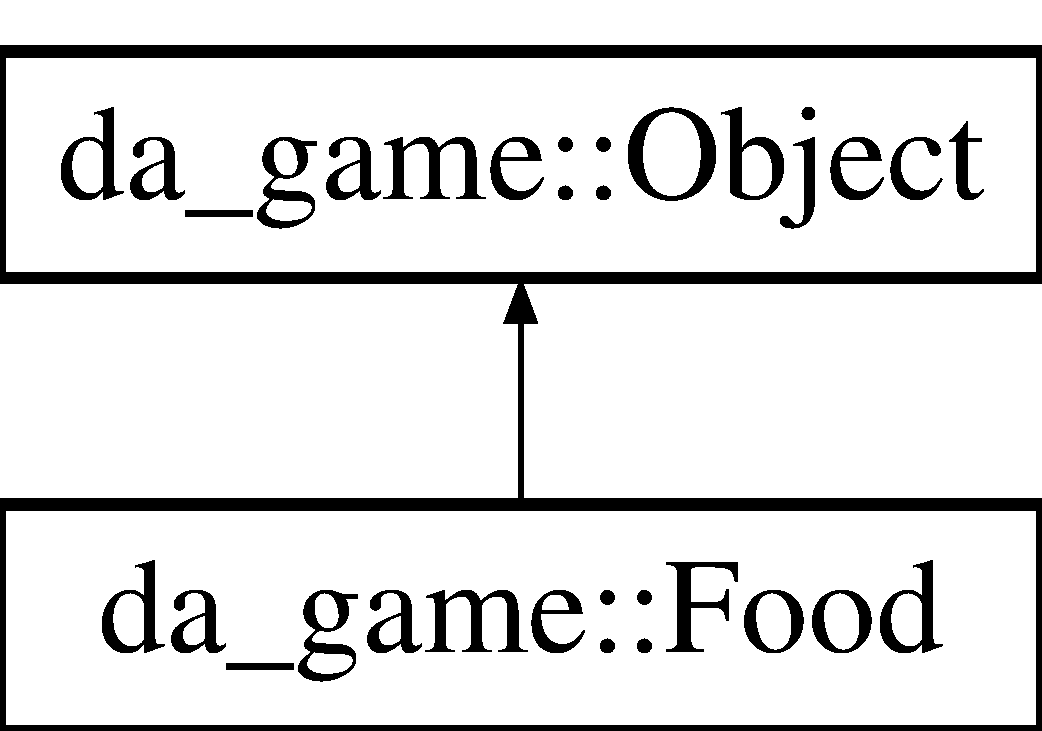
\includegraphics[height=2cm]{classda__game_1_1Food}
\end{center}
\end{figure}
\subsection*{Public Member Functions}
\begin{DoxyCompactItemize}
\item 
\hypertarget{classda__game_1_1Food_ace85d7a8d2b7ae667e8e6d4dc4ec643b}{
{\bfseries Food} (int)}
\label{classda__game_1_1Food_ace85d7a8d2b7ae667e8e6d4dc4ec643b}

\item 
\hypertarget{classda__game_1_1Food_a115b3f00c2184d44adb4252797147f96}{
virtual int {\bfseries health\_\-increase} ()}
\label{classda__game_1_1Food_a115b3f00c2184d44adb4252797147f96}

\item 
\hypertarget{classda__game_1_1Food_a55206a8d4aa3087dce11e629e19befa6}{
virtual int {\bfseries weight} () const }
\label{classda__game_1_1Food_a55206a8d4aa3087dce11e629e19befa6}

\item 
\hypertarget{classda__game_1_1Food_a892fdedaedee16235e95522e618d3631}{
virtual int {\bfseries volume} () const }
\label{classda__game_1_1Food_a892fdedaedee16235e95522e618d3631}

\item 
\hypertarget{classda__game_1_1Food_ad4459dbe0fa30adca487386c91e2a060}{
virtual int {\bfseries price} () const }
\label{classda__game_1_1Food_ad4459dbe0fa30adca487386c91e2a060}

\item 
\hypertarget{classda__game_1_1Food_a0b0cb45b8b004e061a06faf76d6d855d}{
virtual std::string {\bfseries type} () const }
\label{classda__game_1_1Food_a0b0cb45b8b004e061a06faf76d6d855d}

\end{DoxyCompactItemize}
\subsection*{Protected Attributes}
\begin{DoxyCompactItemize}
\item 
\hypertarget{classda__game_1_1Food_ae76b10729eed85aff9a77e6193df89cd}{
int {\bfseries food\_\-left}}
\label{classda__game_1_1Food_ae76b10729eed85aff9a77e6193df89cd}

\end{DoxyCompactItemize}


The documentation for this class was generated from the following files:\begin{DoxyCompactItemize}
\item 
food.h\item 
food.cpp\end{DoxyCompactItemize}

\hypertarget{classda__game_1_1Game}{
\section{da\_\-game::Game Class Reference}
\label{classda__game_1_1Game}\index{da\_\-game::Game@{da\_\-game::Game}}
}
Collaboration diagram for da\_\-game::Game:\nopagebreak
\begin{figure}[H]
\begin{center}
\leavevmode
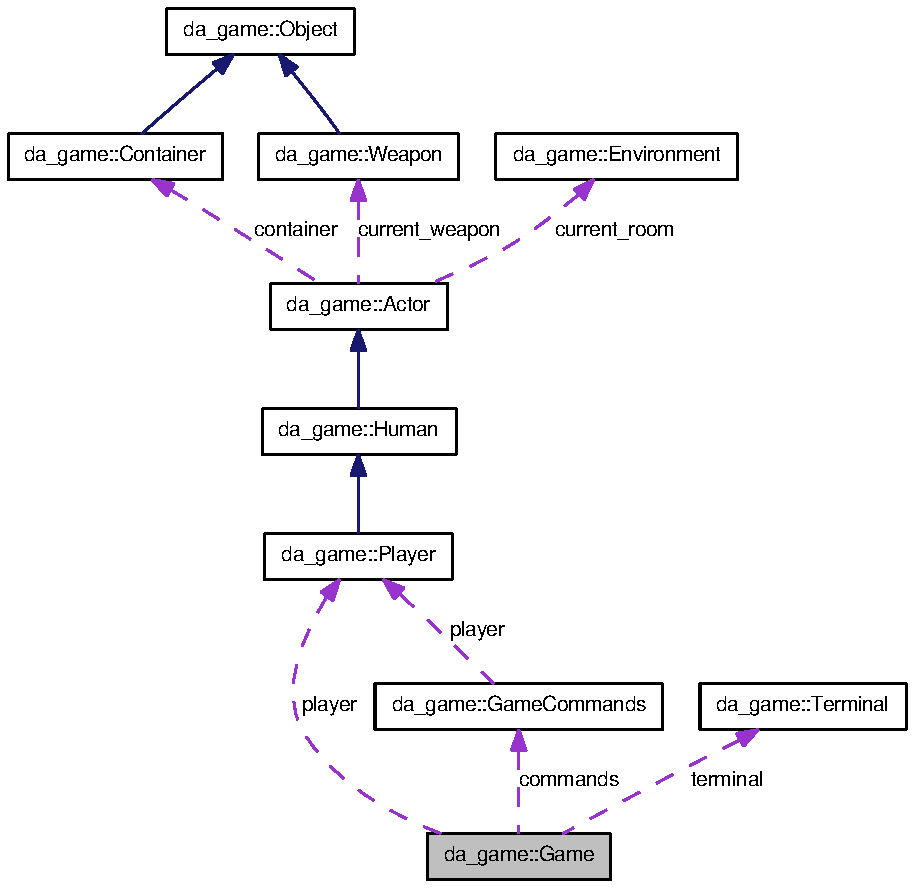
\includegraphics[width=400pt]{classda__game_1_1Game__coll__graph}
\end{center}
\end{figure}
\subsection*{Public Member Functions}
\begin{DoxyCompactItemize}
\item 
\hypertarget{classda__game_1_1Game_aa88f274b8ac3f044da844a0ebc0d9070}{
void {\bfseries initialize} ()}
\label{classda__game_1_1Game_aa88f274b8ac3f044da844a0ebc0d9070}

\end{DoxyCompactItemize}
\subsection*{Static Public Member Functions}
\begin{DoxyCompactItemize}
\item 
\hypertarget{classda__game_1_1Game_a90ae0fd02e47d471a07d1e1958e6e06a}{
static void {\bfseries removeActor} (\hyperlink{classda__game_1_1Actor}{Actor} \&)}
\label{classda__game_1_1Game_a90ae0fd02e47d471a07d1e1958e6e06a}

\end{DoxyCompactItemize}


The documentation for this class was generated from the following files:\begin{DoxyCompactItemize}
\item 
game.h\item 
game.cpp\end{DoxyCompactItemize}

\hypertarget{classda__game_1_1GameCommands}{
\section{da\_\-game::GameCommands Class Reference}
\label{classda__game_1_1GameCommands}\index{da\_\-game::GameCommands@{da\_\-game::GameCommands}}
}
Collaboration diagram for da\_\-game::GameCommands:\nopagebreak
\begin{figure}[H]
\begin{center}
\leavevmode
\includegraphics[width=394pt]{classda__game_1_1GameCommands__coll__graph}
\end{center}
\end{figure}
\subsection*{Public Member Functions}
\begin{DoxyCompactItemize}
\item 
\hypertarget{classda__game_1_1GameCommands_a7f93d626b2cf6b976c49da0a038ef2ea}{
{\bfseries GameCommands} (\hyperlink{classda__game_1_1Player}{Player} $\ast$)}
\label{classda__game_1_1GameCommands_a7f93d626b2cf6b976c49da0a038ef2ea}

\end{DoxyCompactItemize}
\subsection*{Static Public Member Functions}
\begin{DoxyCompactItemize}
\item 
\hypertarget{classda__game_1_1GameCommands_af9378fbac0e9fd15ad39324343f2dd0d}{
static int {\bfseries exit} (std::string)}
\label{classda__game_1_1GameCommands_af9378fbac0e9fd15ad39324343f2dd0d}

\item 
\hypertarget{classda__game_1_1GameCommands_aaca98ea05bd6ecf9671e471a3bd363c7}{
static int {\bfseries go} (std::string)}
\label{classda__game_1_1GameCommands_aaca98ea05bd6ecf9671e471a3bd363c7}

\item 
\hypertarget{classda__game_1_1GameCommands_ad8996732daf4abe8fe1ebebafae2a8de}{
static int {\bfseries fight} (std::string)}
\label{classda__game_1_1GameCommands_ad8996732daf4abe8fe1ebebafae2a8de}

\item 
\hypertarget{classda__game_1_1GameCommands_a8cc72ac921cc6e3a4d95b536e13c03fa}{
static int {\bfseries pick\_\-up} (std::string)}
\label{classda__game_1_1GameCommands_a8cc72ac921cc6e3a4d95b536e13c03fa}

\item 
\hypertarget{classda__game_1_1GameCommands_ae833ca20e0d8171719a70217e990a57c}{
static int {\bfseries drop} (std::string)}
\label{classda__game_1_1GameCommands_ae833ca20e0d8171719a70217e990a57c}

\item 
\hypertarget{classda__game_1_1GameCommands_aa73274bc09851571eaa234a50715624d}{
static int {\bfseries talk\_\-to} (std::string)}
\label{classda__game_1_1GameCommands_aa73274bc09851571eaa234a50715624d}

\item 
\hypertarget{classda__game_1_1GameCommands_a909164da2918f7a7a68fca6c6b698888}{
static int {\bfseries help} (std::string)}
\label{classda__game_1_1GameCommands_a909164da2918f7a7a68fca6c6b698888}

\item 
\hypertarget{classda__game_1_1GameCommands_a49e051175d1bfc13b00c0580e57b07fc}{
static int {\bfseries inventory} (std::string)}
\label{classda__game_1_1GameCommands_a49e051175d1bfc13b00c0580e57b07fc}

\item 
static int \hyperlink{classda__game_1_1GameCommands_a3885d4f3da832d4c06c46f2ad4d14013}{use} (std::string)
\item 
\hypertarget{classda__game_1_1GameCommands_a13f16df34b86dfaf6f21fde3395f356f}{
static void {\bfseries fight} (\hyperlink{classda__game_1_1Actor}{Actor} \&, \hyperlink{classda__game_1_1Actor}{Actor} \&)}
\label{classda__game_1_1GameCommands_a13f16df34b86dfaf6f21fde3395f356f}

\end{DoxyCompactItemize}


\subsection{Member Function Documentation}
\hypertarget{classda__game_1_1GameCommands_a3885d4f3da832d4c06c46f2ad4d14013}{
\index{da\_\-game::GameCommands@{da\_\-game::GameCommands}!use@{use}}
\index{use@{use}!da_game::GameCommands@{da\_\-game::GameCommands}}
\subsubsection[{use}]{\setlength{\rightskip}{0pt plus 5cm}int da\_\-game::GameCommands::use (std::string {\em arg})\hspace{0.3cm}{\ttfamily  \mbox{[}static\mbox{]}}}}
\label{classda__game_1_1GameCommands_a3885d4f3da832d4c06c46f2ad4d14013}
Lets the player use objects, either the objects alone or in combination with other things such as keys on exits.


\begin{DoxyParams}{Parameters}
\item[{\em arg}]The specified argument \end{DoxyParams}
\begin{DoxyReturn}{Returns}
0 if successfully used 
\end{DoxyReturn}


The documentation for this class was generated from the following files:\begin{DoxyCompactItemize}
\item 
game\_\-commands.h\item 
game\_\-commands.cpp\end{DoxyCompactItemize}

\hypertarget{classda__game_1_1Human}{
\section{da\_\-game::Human Class Reference}
\label{classda__game_1_1Human}\index{da\_\-game::Human@{da\_\-game::Human}}
}
Inheritance diagram for da\_\-game::Human:\nopagebreak
\begin{figure}[H]
\begin{center}
\leavevmode
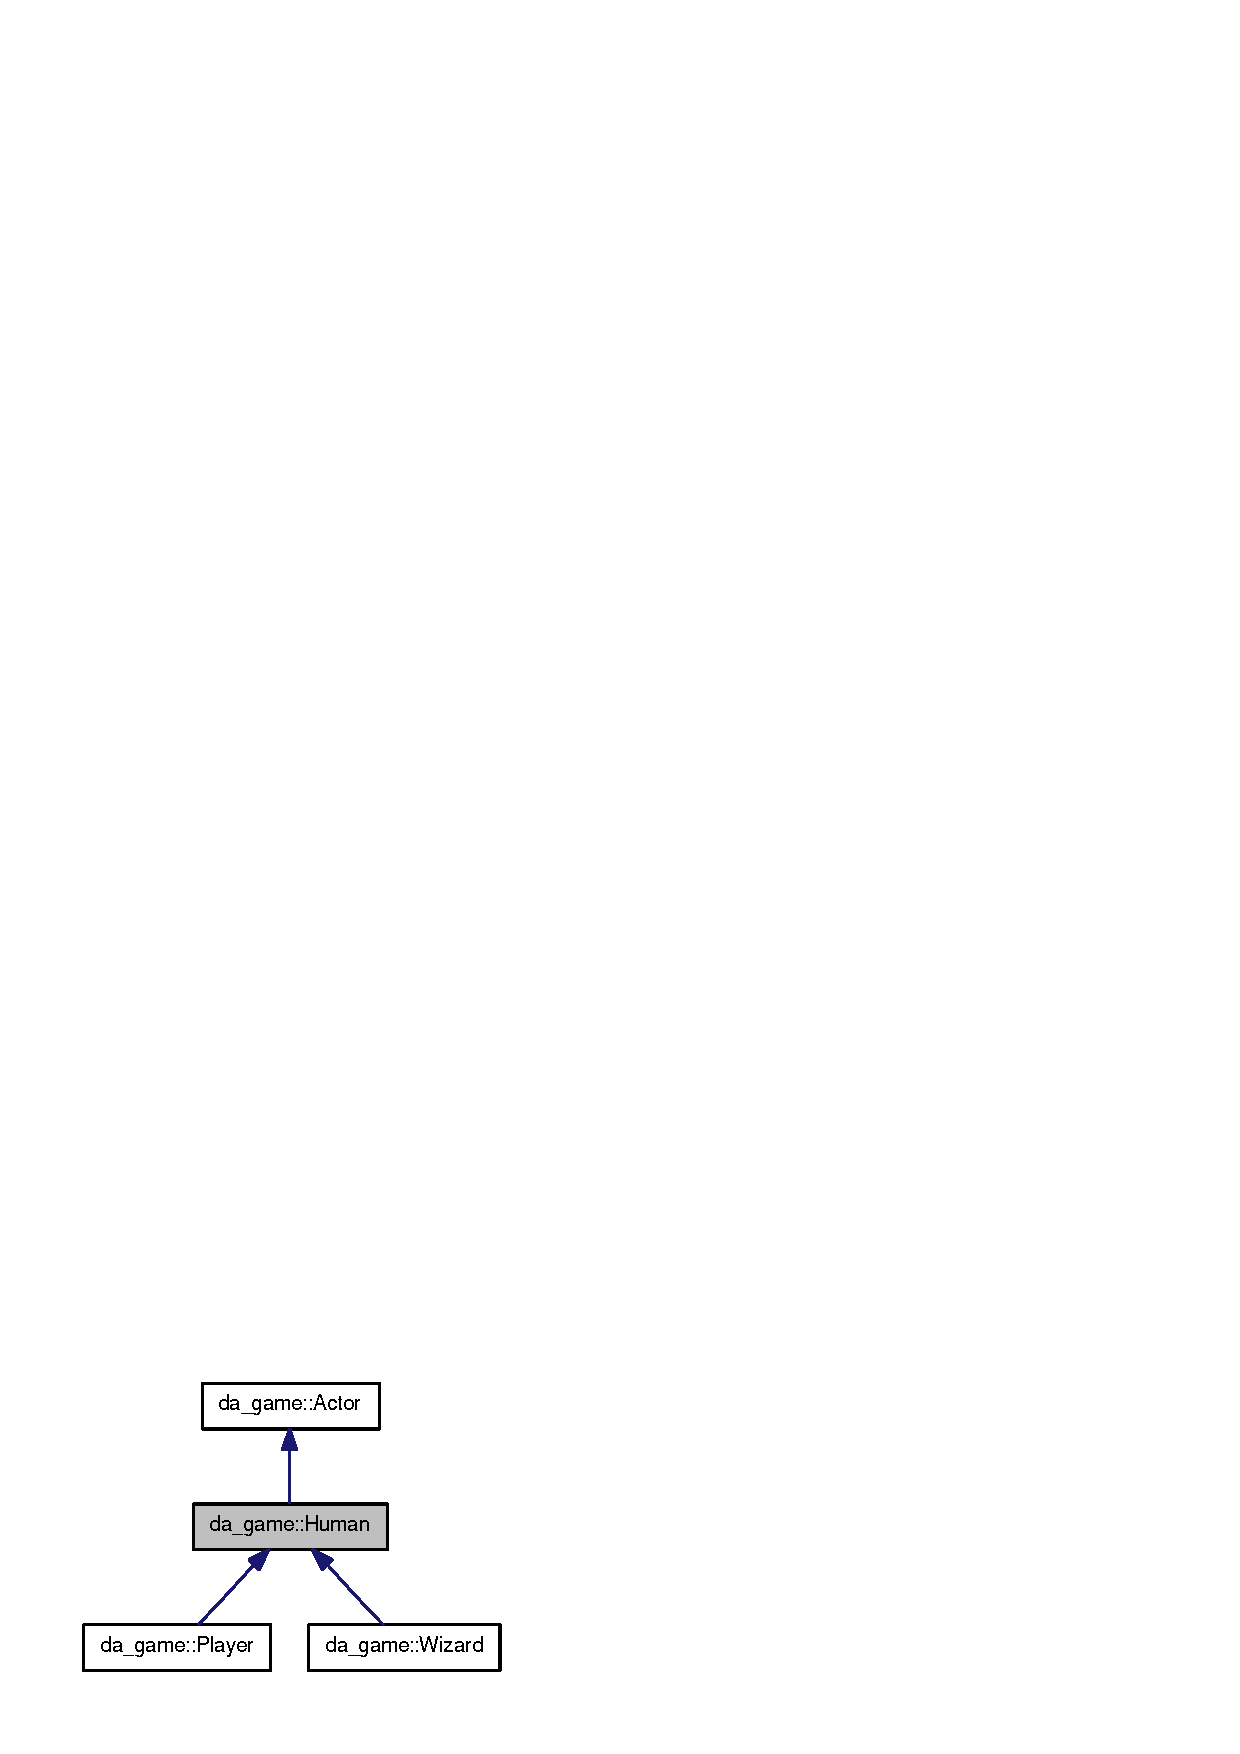
\includegraphics[width=244pt]{classda__game_1_1Human__inherit__graph}
\end{center}
\end{figure}
Collaboration diagram for da\_\-game::Human:\nopagebreak
\begin{figure}[H]
\begin{center}
\leavevmode
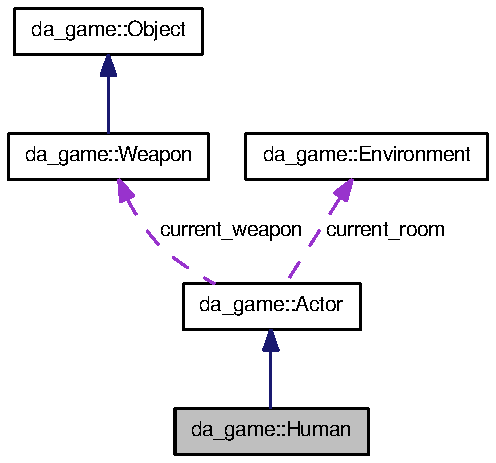
\includegraphics[width=274pt]{classda__game_1_1Human__coll__graph}
\end{center}
\end{figure}
\subsection*{Public Member Functions}
\begin{DoxyCompactItemize}
\item 
\hypertarget{classda__game_1_1Human_aed0a521eea5a8fa1cce0bc0accd616ae}{
{\bfseries Human} (bool, int)}
\label{classda__game_1_1Human_aed0a521eea5a8fa1cce0bc0accd616ae}

\item 
\hypertarget{classda__game_1_1Human_a7861ade5e3d97c1945690f961f6aa2f0}{
virtual void {\bfseries run} ()}
\label{classda__game_1_1Human_a7861ade5e3d97c1945690f961f6aa2f0}

\item 
\hypertarget{classda__game_1_1Human_ae8cf665bea081f6eb7cb9889e77ceafb}{
virtual std::string {\bfseries get\_\-type} () const }
\label{classda__game_1_1Human_ae8cf665bea081f6eb7cb9889e77ceafb}

\item 
\hypertarget{classda__game_1_1Human_a2700b5d52961ba140d14d4da246b1a77}{
void {\bfseries eat} (\hyperlink{classda__game_1_1Food}{Food} \&)}
\label{classda__game_1_1Human_a2700b5d52961ba140d14d4da246b1a77}

\end{DoxyCompactItemize}
\subsection*{Protected Attributes}
\begin{DoxyCompactItemize}
\item 
\hypertarget{classda__game_1_1Human_a1b81e3167c625be17bb25e1edf273a77}{
bool {\bfseries has\_\-heart}}
\label{classda__game_1_1Human_a1b81e3167c625be17bb25e1edf273a77}

\item 
\hypertarget{classda__game_1_1Human_a4e47ed43e00e5604e671e432c008d764}{
int {\bfseries max\_\-health}}
\label{classda__game_1_1Human_a4e47ed43e00e5604e671e432c008d764}

\end{DoxyCompactItemize}


The documentation for this class was generated from the following files:\begin{DoxyCompactItemize}
\item 
human.h\item 
human.cpp\end{DoxyCompactItemize}

\hypertarget{classda__game_1_1Inside}{
\section{da\_\-game::Inside Class Reference}
\label{classda__game_1_1Inside}\index{da\_\-game::Inside@{da\_\-game::Inside}}
}
Inheritance diagram for da\_\-game::Inside:\nopagebreak
\begin{figure}[H]
\begin{center}
\leavevmode
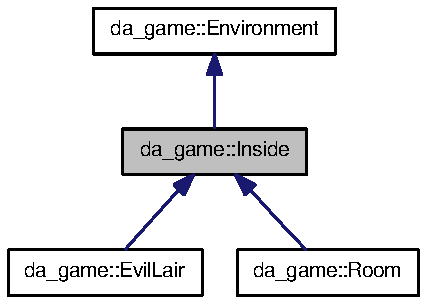
\includegraphics[width=240pt]{classda__game_1_1Inside__inherit__graph}
\end{center}
\end{figure}
Collaboration diagram for da\_\-game::Inside:\nopagebreak
\begin{figure}[H]
\begin{center}
\leavevmode
\includegraphics[width=160pt]{classda__game_1_1Inside__coll__graph}
\end{center}
\end{figure}
\subsection*{Public Member Functions}
\begin{DoxyCompactItemize}
\item 
\hyperlink{classda__game_1_1Inside_a90752ab2ce2d5991185aba47e962befd}{Inside} ()
\item 
\hyperlink{classda__game_1_1Inside_aa36eb3ecd2ad203540866314d5392078}{Inside} (\hyperlink{classda__game_1_1Exit}{Exit} $\ast$, \hyperlink{classda__game_1_1Exit}{Exit} $\ast$, \hyperlink{classda__game_1_1Exit}{Exit} $\ast$, \hyperlink{classda__game_1_1Exit}{Exit} $\ast$)
\end{DoxyCompactItemize}


\subsection{Constructor \& Destructor Documentation}
\hypertarget{classda__game_1_1Inside_a90752ab2ce2d5991185aba47e962befd}{
\index{da\_\-game::Inside@{da\_\-game::Inside}!Inside@{Inside}}
\index{Inside@{Inside}!da_game::Inside@{da\_\-game::Inside}}
\subsubsection[{Inside}]{\setlength{\rightskip}{0pt plus 5cm}da\_\-game::Inside::Inside ()}}
\label{classda__game_1_1Inside_a90752ab2ce2d5991185aba47e962befd}
Constructs a new empty inside environment with no exits. \hypertarget{classda__game_1_1Inside_aa36eb3ecd2ad203540866314d5392078}{
\index{da\_\-game::Inside@{da\_\-game::Inside}!Inside@{Inside}}
\index{Inside@{Inside}!da_game::Inside@{da\_\-game::Inside}}
\subsubsection[{Inside}]{\setlength{\rightskip}{0pt plus 5cm}da\_\-game::Inside::Inside ({\bf Exit} $\ast$ {\em east}, \/  {\bf Exit} $\ast$ {\em west}, \/  {\bf Exit} $\ast$ {\em north}, \/  {\bf Exit} $\ast$ {\em south})}}
\label{classda__game_1_1Inside_aa36eb3ecd2ad203540866314d5392078}
Constructs a new inside environment.


\begin{DoxyParams}{Parameters}
\item[{\em east}]The east exit \item[{\em west}]The west exit \item[{\em north}]The north exit \item[{\em south}]The south exit \end{DoxyParams}


The documentation for this class was generated from the following files:\begin{DoxyCompactItemize}
\item 
inside.h\item 
inside.cpp\end{DoxyCompactItemize}

\hypertarget{classda__game_1_1Key}{
\section{da\_\-game::Key Class Reference}
\label{classda__game_1_1Key}\index{da\_\-game::Key@{da\_\-game::Key}}
}


{\ttfamily \#include $<$key.h$>$}Inheritance diagram for da\_\-game::Key:\nopagebreak
\begin{figure}[H]
\begin{center}
\leavevmode
\includegraphics[width=134pt]{classda__game_1_1Key__inherit__graph}
\end{center}
\end{figure}
Collaboration diagram for da\_\-game::Key:\nopagebreak
\begin{figure}[H]
\begin{center}
\leavevmode
\includegraphics[width=134pt]{classda__game_1_1Key__coll__graph}
\end{center}
\end{figure}
\subsection*{Public Member Functions}
\begin{DoxyCompactItemize}
\item 
\hyperlink{classda__game_1_1Key_a15fcc235eb6d5c76e574fd02ab9bad4b}{Key} (std::string)
\item 
virtual int \hyperlink{classda__game_1_1Key_a3a55f412166c6da8d3919978edb214e5}{weight} () const 
\item 
virtual int \hyperlink{classda__game_1_1Key_ac21b171678f19465b41796007896dc84}{volume} () const 
\item 
virtual int \hyperlink{classda__game_1_1Key_af9752b65636483258a50e7ae553d131a}{price} () const 
\item 
virtual std::string \hyperlink{classda__game_1_1Key_adaecf6030e14cd4da5142e8c760c5741}{type} () const 
\item 
virtual bool \hyperlink{classda__game_1_1Key_af3b5c0256dfcfc935e898d27dd47ffeb}{operator==} (\hyperlink{classda__game_1_1Key}{Key} \&) const 
\item 
std::string \hyperlink{classda__game_1_1Key_a1d96d265ce05db8566dfd62615de61c6}{get\_\-key\_\-code} () const 
\end{DoxyCompactItemize}


\subsection{Detailed Description}
A key may be used for locking and unlocking doors. It utilises a special keycode which has to agree with the corresponding code for the door. 

\subsection{Constructor \& Destructor Documentation}
\hypertarget{classda__game_1_1Key_a15fcc235eb6d5c76e574fd02ab9bad4b}{
\index{da\_\-game::Key@{da\_\-game::Key}!Key@{Key}}
\index{Key@{Key}!da_game::Key@{da\_\-game::Key}}
\subsubsection[{Key}]{\setlength{\rightskip}{0pt plus 5cm}da\_\-game::Key::Key (std::string {\em key\_\-code})}}
\label{classda__game_1_1Key_a15fcc235eb6d5c76e574fd02ab9bad4b}
Creates a new key with the given key code.


\begin{DoxyParams}{Parameters}
\item[{\em key\_\-code}]The key code for this key \end{DoxyParams}


\subsection{Member Function Documentation}
\hypertarget{classda__game_1_1Key_a1d96d265ce05db8566dfd62615de61c6}{
\index{da\_\-game::Key@{da\_\-game::Key}!get\_\-key\_\-code@{get\_\-key\_\-code}}
\index{get\_\-key\_\-code@{get\_\-key\_\-code}!da_game::Key@{da\_\-game::Key}}
\subsubsection[{get\_\-key\_\-code}]{\setlength{\rightskip}{0pt plus 5cm}std::string da\_\-game::Key::get\_\-key\_\-code () const}}
\label{classda__game_1_1Key_a1d96d265ce05db8566dfd62615de61c6}
Returns the key code of this key.

\begin{DoxyReturn}{Returns}
the key code 
\end{DoxyReturn}
\hypertarget{classda__game_1_1Key_af3b5c0256dfcfc935e898d27dd47ffeb}{
\index{da\_\-game::Key@{da\_\-game::Key}!operator==@{operator==}}
\index{operator==@{operator==}!da_game::Key@{da\_\-game::Key}}
\subsubsection[{operator==}]{\setlength{\rightskip}{0pt plus 5cm}bool da\_\-game::Key::operator== ({\bf Key} \& {\em key}) const\hspace{0.3cm}{\ttfamily  \mbox{[}virtual\mbox{]}}}}
\label{classda__game_1_1Key_af3b5c0256dfcfc935e898d27dd47ffeb}
Compares the specified object to this key and returns true if they are considered equal. In this case they are considered equal if and only if the specified object is also a key and all of its parameters coincide with the ones of this key.

\begin{DoxyReturn}{Returns}
true iff the object is identically equal to this key 
\end{DoxyReturn}


Reimplemented from \hyperlink{classda__game_1_1Object}{da\_\-game::Object}.\hypertarget{classda__game_1_1Key_af9752b65636483258a50e7ae553d131a}{
\index{da\_\-game::Key@{da\_\-game::Key}!price@{price}}
\index{price@{price}!da_game::Key@{da\_\-game::Key}}
\subsubsection[{price}]{\setlength{\rightskip}{0pt plus 5cm}int da\_\-game::Key::price () const\hspace{0.3cm}{\ttfamily  \mbox{[}virtual\mbox{]}}}}
\label{classda__game_1_1Key_af9752b65636483258a50e7ae553d131a}
Returns the price of this key.

\begin{DoxyReturn}{Returns}
the price 
\end{DoxyReturn}


Implements \hyperlink{classda__game_1_1Object}{da\_\-game::Object}.\hypertarget{classda__game_1_1Key_adaecf6030e14cd4da5142e8c760c5741}{
\index{da\_\-game::Key@{da\_\-game::Key}!type@{type}}
\index{type@{type}!da_game::Key@{da\_\-game::Key}}
\subsubsection[{type}]{\setlength{\rightskip}{0pt plus 5cm}std::string da\_\-game::Key::type () const\hspace{0.3cm}{\ttfamily  \mbox{[}virtual\mbox{]}}}}
\label{classda__game_1_1Key_adaecf6030e14cd4da5142e8c760c5741}
Returns the type of this key.

\begin{DoxyReturn}{Returns}
the type 
\end{DoxyReturn}


Implements \hyperlink{classda__game_1_1Object}{da\_\-game::Object}.\hypertarget{classda__game_1_1Key_ac21b171678f19465b41796007896dc84}{
\index{da\_\-game::Key@{da\_\-game::Key}!volume@{volume}}
\index{volume@{volume}!da_game::Key@{da\_\-game::Key}}
\subsubsection[{volume}]{\setlength{\rightskip}{0pt plus 5cm}int da\_\-game::Key::volume () const\hspace{0.3cm}{\ttfamily  \mbox{[}virtual\mbox{]}}}}
\label{classda__game_1_1Key_ac21b171678f19465b41796007896dc84}
Returns the volume of this key.

\begin{DoxyReturn}{Returns}
the volume 
\end{DoxyReturn}


Implements \hyperlink{classda__game_1_1Object}{da\_\-game::Object}.\hypertarget{classda__game_1_1Key_a3a55f412166c6da8d3919978edb214e5}{
\index{da\_\-game::Key@{da\_\-game::Key}!weight@{weight}}
\index{weight@{weight}!da_game::Key@{da\_\-game::Key}}
\subsubsection[{weight}]{\setlength{\rightskip}{0pt plus 5cm}int da\_\-game::Key::weight () const\hspace{0.3cm}{\ttfamily  \mbox{[}virtual\mbox{]}}}}
\label{classda__game_1_1Key_a3a55f412166c6da8d3919978edb214e5}
Returns the weight of this key.

\begin{DoxyReturn}{Returns}
the weight 
\end{DoxyReturn}


Implements \hyperlink{classda__game_1_1Object}{da\_\-game::Object}.

The documentation for this class was generated from the following files:\begin{DoxyCompactItemize}
\item 
key.h\item 
key.cpp\end{DoxyCompactItemize}

\hypertarget{classda__game_1_1LightSaber}{
\section{da\_\-game::LightSaber Class Reference}
\label{classda__game_1_1LightSaber}\index{da\_\-game::LightSaber@{da\_\-game::LightSaber}}
}
Inheritance diagram for da\_\-game::LightSaber:\nopagebreak
\begin{figure}[H]
\begin{center}
\leavevmode
\includegraphics[width=152pt]{classda__game_1_1LightSaber__inherit__graph}
\end{center}
\end{figure}
Collaboration diagram for da\_\-game::LightSaber:\nopagebreak
\begin{figure}[H]
\begin{center}
\leavevmode
\includegraphics[width=152pt]{classda__game_1_1LightSaber__coll__graph}
\end{center}
\end{figure}
\subsection*{Public Member Functions}
\begin{DoxyCompactItemize}
\item 
\hypertarget{classda__game_1_1LightSaber_a4008857749873e2a2cd3bc8258e05741}{
{\bfseries LightSaber} (unsigned int, float)}
\label{classda__game_1_1LightSaber_a4008857749873e2a2cd3bc8258e05741}

\item 
\hypertarget{classda__game_1_1LightSaber_aa4ca392fb17a006df70176045e36ba4d}{
virtual int {\bfseries weight} () const }
\label{classda__game_1_1LightSaber_aa4ca392fb17a006df70176045e36ba4d}

\item 
\hypertarget{classda__game_1_1LightSaber_ab2883eb294fb19ac5bbb9c5215f1cfd5}{
virtual int {\bfseries volume} () const }
\label{classda__game_1_1LightSaber_ab2883eb294fb19ac5bbb9c5215f1cfd5}

\item 
\hypertarget{classda__game_1_1LightSaber_a2ddf499cbf92bb6456beac3b4b6bcd64}{
virtual int {\bfseries price} () const }
\label{classda__game_1_1LightSaber_a2ddf499cbf92bb6456beac3b4b6bcd64}

\item 
\hypertarget{classda__game_1_1LightSaber_ac69f6a976779c9c16d48ee7637a4a8db}{
virtual std::string {\bfseries type} () const }
\label{classda__game_1_1LightSaber_ac69f6a976779c9c16d48ee7637a4a8db}

\end{DoxyCompactItemize}


The documentation for this class was generated from the following files:\begin{DoxyCompactItemize}
\item 
light\_\-saber.h\item 
light\_\-saber.cpp\end{DoxyCompactItemize}

\hypertarget{classda__game_1_1Object}{
\section{da\_\-game::Object Class Reference}
\label{classda__game_1_1Object}\index{da\_\-game::Object@{da\_\-game::Object}}
}
Inheritance diagram for da\_\-game::Object::\begin{figure}[H]
\begin{center}
\leavevmode
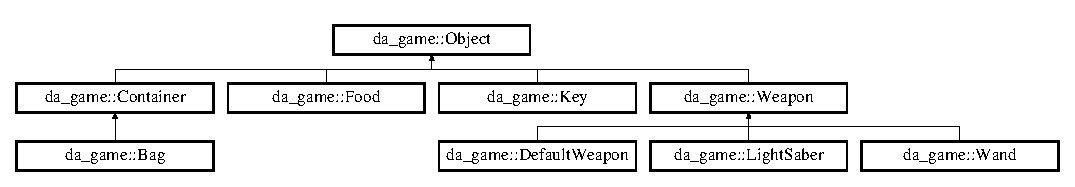
\includegraphics[height=2.06135cm]{classda__game_1_1Object}
\end{center}
\end{figure}
\subsection*{Public Member Functions}
\begin{DoxyCompactItemize}
\item 
\hypertarget{classda__game_1_1Object_af8bc16da0544770ea56f9fc4b60d2d7a}{
virtual int {\bfseries weight} () const =0}
\label{classda__game_1_1Object_af8bc16da0544770ea56f9fc4b60d2d7a}

\item 
\hypertarget{classda__game_1_1Object_a725094f0008c07a674acf3eb042d457e}{
virtual int {\bfseries volume} () const =0}
\label{classda__game_1_1Object_a725094f0008c07a674acf3eb042d457e}

\item 
\hypertarget{classda__game_1_1Object_a8ffadf9d43a195e7ac69b80963833a4d}{
virtual int {\bfseries price} () const =0}
\label{classda__game_1_1Object_a8ffadf9d43a195e7ac69b80963833a4d}

\item 
\hypertarget{classda__game_1_1Object_a2571d77aaf04c5be1f6556c4c7bab0d2}{
virtual std::string {\bfseries type} () const =0}
\label{classda__game_1_1Object_a2571d77aaf04c5be1f6556c4c7bab0d2}

\item 
\hypertarget{classda__game_1_1Object_a73b5e428218a64db3e84df9f016352c2}{
virtual bool {\bfseries operator==} (\hyperlink{classda__game_1_1Object}{Object} \&) const }
\label{classda__game_1_1Object_a73b5e428218a64db3e84df9f016352c2}

\end{DoxyCompactItemize}
\subsection*{Public Attributes}
\begin{DoxyCompactItemize}
\item 
\hypertarget{classda__game_1_1Object_ab2a154b5ce3c8e9acb7e60614687d704}{
const int {\bfseries id}}
\label{classda__game_1_1Object_ab2a154b5ce3c8e9acb7e60614687d704}

\end{DoxyCompactItemize}
\subsection*{Static Protected Attributes}
\begin{DoxyCompactItemize}
\item 
\hypertarget{classda__game_1_1Object_a696eccdeb3f9d1df936ee93aeb1da16f}{
static int {\bfseries instances}}
\label{classda__game_1_1Object_a696eccdeb3f9d1df936ee93aeb1da16f}

\end{DoxyCompactItemize}


The documentation for this class was generated from the following files:\begin{DoxyCompactItemize}
\item 
object.h\item 
object.cpp\end{DoxyCompactItemize}

\hypertarget{classda__game_1_1Outside}{
\section{da\_\-game::Outside Class Reference}
\label{classda__game_1_1Outside}\index{da\_\-game::Outside@{da\_\-game::Outside}}
}
Inheritance diagram for da\_\-game::Outside::\begin{figure}[H]
\begin{center}
\leavevmode
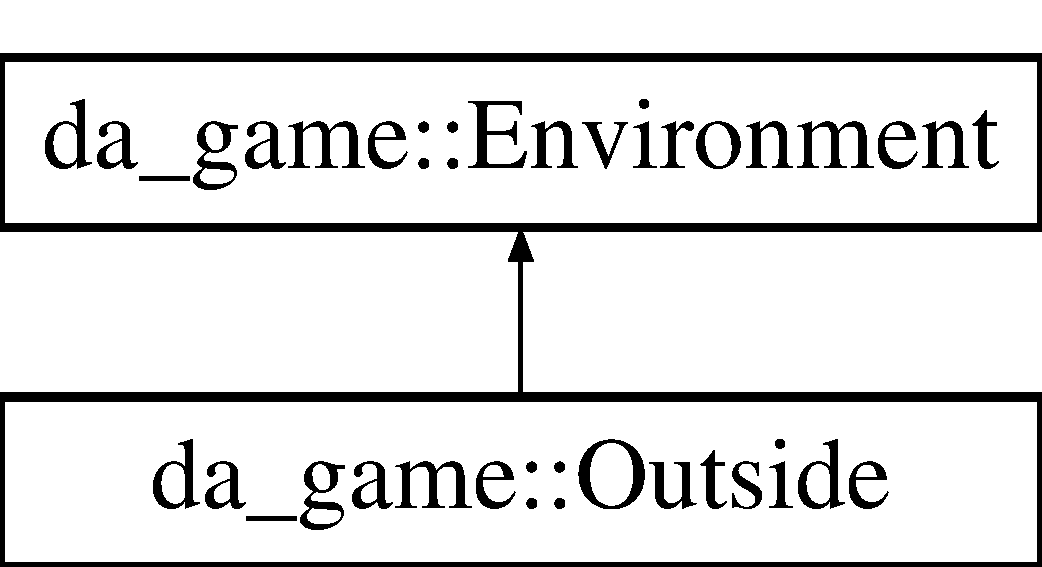
\includegraphics[height=2cm]{classda__game_1_1Outside}
\end{center}
\end{figure}


The documentation for this class was generated from the following file:\begin{DoxyCompactItemize}
\item 
outside.h\end{DoxyCompactItemize}

\hypertarget{classda__game_1_1Player}{
\section{da\_\-game::Player Class Reference}
\label{classda__game_1_1Player}\index{da\_\-game::Player@{da\_\-game::Player}}
}
Inheritance diagram for da\_\-game::Player:\nopagebreak
\begin{figure}[H]
\begin{center}
\leavevmode
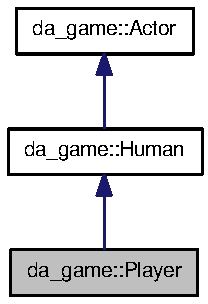
\includegraphics[width=136pt]{classda__game_1_1Player__inherit__graph}
\end{center}
\end{figure}
Collaboration diagram for da\_\-game::Player:\nopagebreak
\begin{figure}[H]
\begin{center}
\leavevmode
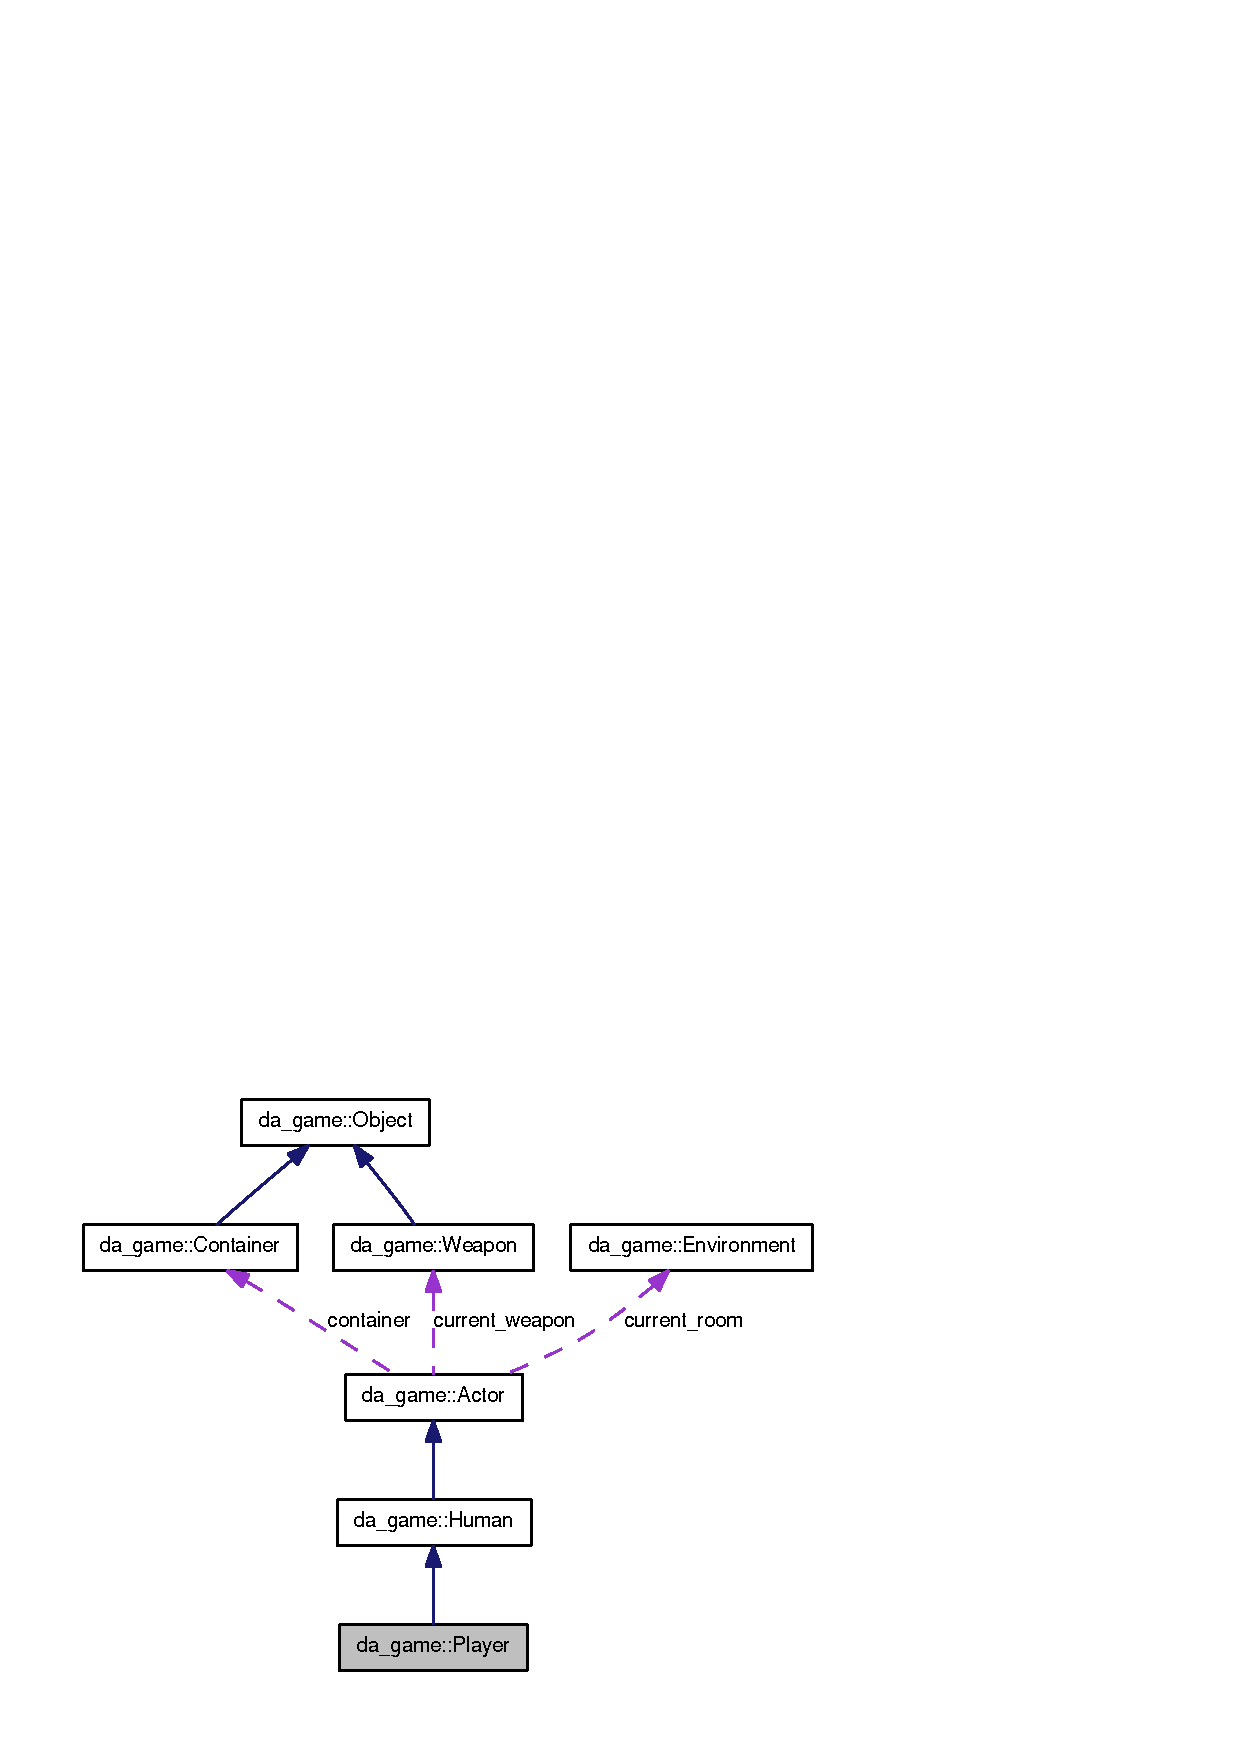
\includegraphics[width=274pt]{classda__game_1_1Player__coll__graph}
\end{center}
\end{figure}
\subsection*{Public Member Functions}
\begin{DoxyCompactItemize}
\item 
\hypertarget{classda__game_1_1Player_a9595c922f10179598390ceb4015bd2f4}{
{\bfseries Player} (\hyperlink{classda__game_1_1Environment}{Environment} $\ast$)}
\label{classda__game_1_1Player_a9595c922f10179598390ceb4015bd2f4}

\item 
\hypertarget{classda__game_1_1Player_a82953e4dd060cc994a466cc4396416bc}{
virtual void {\bfseries run} ()}
\label{classda__game_1_1Player_a82953e4dd060cc994a466cc4396416bc}

\item 
\hypertarget{classda__game_1_1Player_a3a7221090c308a8a72ef464b06f805a4}{
virtual std::string {\bfseries get\_\-type} () const }
\label{classda__game_1_1Player_a3a7221090c308a8a72ef464b06f805a4}

\item 
\hypertarget{classda__game_1_1Player_ac4525d9ce538a66f6f97678e20310e5e}{
virtual std::string {\bfseries get\_\-name} () const }
\label{classda__game_1_1Player_ac4525d9ce538a66f6f97678e20310e5e}

\item 
\hypertarget{classda__game_1_1Player_aff77ce1e994cf473bb35a2341f937f89}{
virtual void {\bfseries fight} (\hyperlink{classda__game_1_1Actor}{Actor} \&)}
\label{classda__game_1_1Player_aff77ce1e994cf473bb35a2341f937f89}

\item 
\hypertarget{classda__game_1_1Player_a6c0c3861b261abc16292c6bc74fbe39b}{
virtual void {\bfseries talk\_\-to} (\hyperlink{classda__game_1_1Actor}{Actor} \&)}
\label{classda__game_1_1Player_a6c0c3861b261abc16292c6bc74fbe39b}

\item 
\hypertarget{classda__game_1_1Player_a1bf7665cb71afb0d63c0c264496e9b44}{
virtual \hyperlink{classda__game_1_1Environment}{Environment} $\ast$ {\bfseries get\_\-room} () const }
\label{classda__game_1_1Player_a1bf7665cb71afb0d63c0c264496e9b44}

\end{DoxyCompactItemize}
\subsection*{Friends}
\begin{DoxyCompactItemize}
\item 
\hypertarget{classda__game_1_1Player_ad58162d418e52e78ef2d13bea08472d4}{
class {\bfseries GameCommands}}
\label{classda__game_1_1Player_ad58162d418e52e78ef2d13bea08472d4}

\end{DoxyCompactItemize}


The documentation for this class was generated from the following files:\begin{DoxyCompactItemize}
\item 
player.h\item 
player.cpp\end{DoxyCompactItemize}

\hypertarget{classda__game_1_1Room}{
\section{da\_\-game::Room Class Reference}
\label{classda__game_1_1Room}\index{da\_\-game::Room@{da\_\-game::Room}}
}
Inheritance diagram for da\_\-game::Room:\nopagebreak
\begin{figure}[H]
\begin{center}
\leavevmode
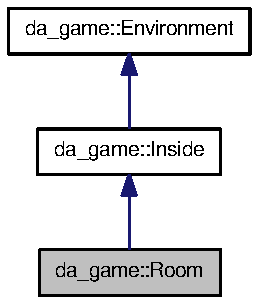
\includegraphics[width=160pt]{classda__game_1_1Room__inherit__graph}
\end{center}
\end{figure}
Collaboration diagram for da\_\-game::Room:\nopagebreak
\begin{figure}[H]
\begin{center}
\leavevmode
\includegraphics[width=160pt]{classda__game_1_1Room__coll__graph}
\end{center}
\end{figure}
\subsection*{Public Member Functions}
\begin{DoxyCompactItemize}
\item 
\hyperlink{classda__game_1_1Room_aa36091a4e06c697468cd4e48da7d94c1}{Room} ()
\item 
\hyperlink{classda__game_1_1Room_ac8abf8b2bb0499d4008859ba8a5bb3d3}{Room} (\hyperlink{classda__game_1_1Exit}{Exit} $\ast$, \hyperlink{classda__game_1_1Exit}{Exit} $\ast$, \hyperlink{classda__game_1_1Exit}{Exit} $\ast$, \hyperlink{classda__game_1_1Exit}{Exit} $\ast$)
\item 
\hypertarget{classda__game_1_1Room_a7fabe80fe90a22324aeda1aa3a315903}{
virtual std::string {\bfseries description} () const }
\label{classda__game_1_1Room_a7fabe80fe90a22324aeda1aa3a315903}

\end{DoxyCompactItemize}


\subsection{Constructor \& Destructor Documentation}
\hypertarget{classda__game_1_1Room_aa36091a4e06c697468cd4e48da7d94c1}{
\index{da\_\-game::Room@{da\_\-game::Room}!Room@{Room}}
\index{Room@{Room}!da_game::Room@{da\_\-game::Room}}
\subsubsection[{Room}]{\setlength{\rightskip}{0pt plus 5cm}da\_\-game::Room::Room ()}}
\label{classda__game_1_1Room_aa36091a4e06c697468cd4e48da7d94c1}
Constructs an empty room with no exits. \hypertarget{classda__game_1_1Room_ac8abf8b2bb0499d4008859ba8a5bb3d3}{
\index{da\_\-game::Room@{da\_\-game::Room}!Room@{Room}}
\index{Room@{Room}!da_game::Room@{da\_\-game::Room}}
\subsubsection[{Room}]{\setlength{\rightskip}{0pt plus 5cm}da\_\-game::Room::Room ({\bf Exit} $\ast$ {\em east}, \/  {\bf Exit} $\ast$ {\em west}, \/  {\bf Exit} $\ast$ {\em north}, \/  {\bf Exit} $\ast$ {\em south})}}
\label{classda__game_1_1Room_ac8abf8b2bb0499d4008859ba8a5bb3d3}
Constructs a new room with the specified exits. 

The documentation for this class was generated from the following files:\begin{DoxyCompactItemize}
\item 
room.h\item 
room.cpp\end{DoxyCompactItemize}

\hypertarget{classda__game_1_1Terminal}{
\section{da\_\-game::Terminal Class Reference}
\label{classda__game_1_1Terminal}\index{da\_\-game::Terminal@{da\_\-game::Terminal}}
}
\subsection*{Public Member Functions}
\begin{DoxyCompactItemize}
\item 
\hypertarget{classda__game_1_1Terminal_a2332b0a1f5af08b26d0a6ab6995af624}{
int {\bfseries run} ()}
\label{classda__game_1_1Terminal_a2332b0a1f5af08b26d0a6ab6995af624}

\end{DoxyCompactItemize}
\subsection*{Static Public Member Functions}
\begin{DoxyCompactItemize}
\item 
\hypertarget{classda__game_1_1Terminal_ae04f49aa880c92ab3046e38bffda825e}{
static bool {\bfseries add\_\-function} (std::string, int($\ast$)(std::string))}
\label{classda__game_1_1Terminal_ae04f49aa880c92ab3046e38bffda825e}

\item 
\hypertarget{classda__game_1_1Terminal_ab97f45258ad52ebdf946a2e0a9434c66}{
static const std::map$<$ std::string, int($\ast$ {\bfseries get\_\-functions} ())(std::string)$>$}
\label{classda__game_1_1Terminal_ab97f45258ad52ebdf946a2e0a9434c66}

\item 
\hypertarget{classda__game_1_1Terminal_a5d545f56be7d990ce0c77a2fe8cd5042}{
static void {\bfseries print} (std::string)}
\label{classda__game_1_1Terminal_a5d545f56be7d990ce0c77a2fe8cd5042}

\end{DoxyCompactItemize}


The documentation for this class was generated from the following files:\begin{DoxyCompactItemize}
\item 
terminal.h\item 
terminal.cpp\end{DoxyCompactItemize}

\hypertarget{classda__game_1_1Troll}{
\section{da\_\-game::Troll Class Reference}
\label{classda__game_1_1Troll}\index{da\_\-game::Troll@{da\_\-game::Troll}}
}
Inheritance diagram for da\_\-game::Troll::\begin{figure}[H]
\begin{center}
\leavevmode
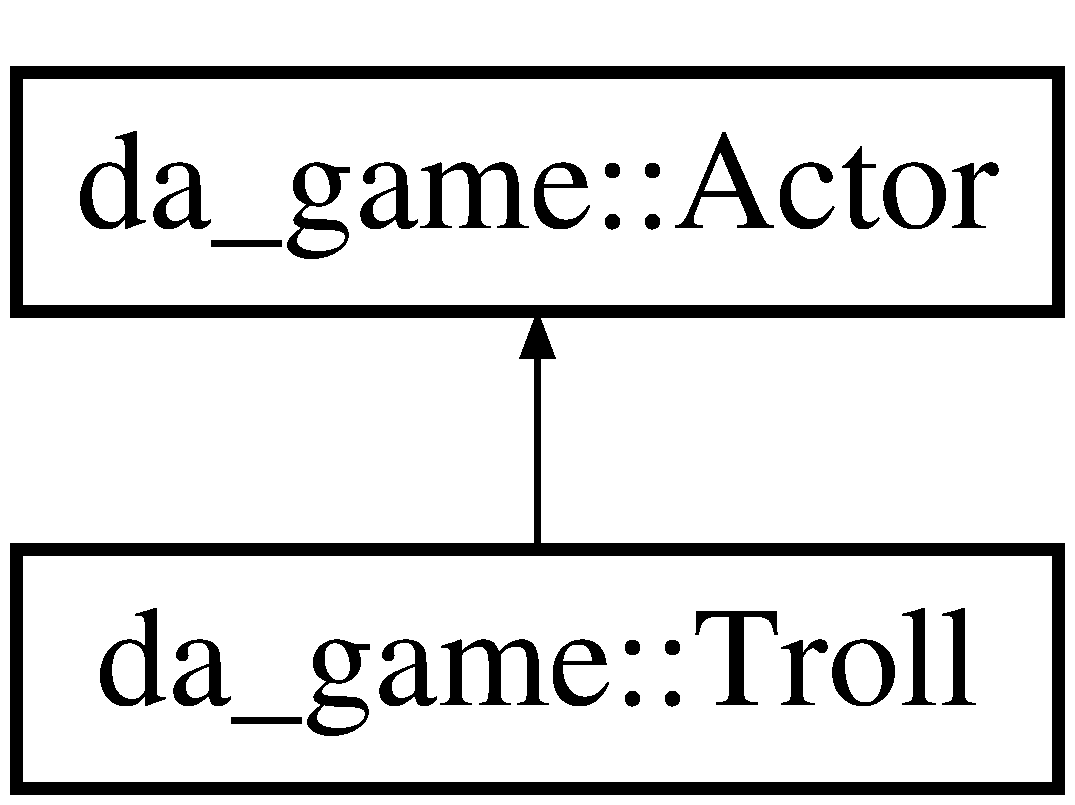
\includegraphics[height=2cm]{classda__game_1_1Troll}
\end{center}
\end{figure}
\subsection*{Public Member Functions}
\begin{DoxyCompactItemize}
\item 
\hypertarget{classda__game_1_1Troll_a7b6cee5ab1339572982aa4f490b09b65}{
{\bfseries Troll} (\hyperlink{classda__game_1_1Environment}{Environment} $\ast$, int, int)}
\label{classda__game_1_1Troll_a7b6cee5ab1339572982aa4f490b09b65}

\item 
\hypertarget{classda__game_1_1Troll_a5ff7be42450036dee76060892ed52dd6}{
void {\bfseries eat} (\hyperlink{classda__game_1_1Actor}{Actor} \&)}
\label{classda__game_1_1Troll_a5ff7be42450036dee76060892ed52dd6}

\item 
\hypertarget{classda__game_1_1Troll_a50a5ca63166711c2ce631c6ec5cd2cad}{
void {\bfseries eat} (\hyperlink{classda__game_1_1Food}{Food} \&)}
\label{classda__game_1_1Troll_a50a5ca63166711c2ce631c6ec5cd2cad}

\item 
\hypertarget{classda__game_1_1Troll_a52d102598f13c6dea7311cc16d8bbc50}{
virtual void {\bfseries run} ()}
\label{classda__game_1_1Troll_a52d102598f13c6dea7311cc16d8bbc50}

\item 
\hypertarget{classda__game_1_1Troll_ac00b5c9350f950390cef9fcb365fd4e2}{
virtual std::string {\bfseries get\_\-type} () const }
\label{classda__game_1_1Troll_ac00b5c9350f950390cef9fcb365fd4e2}

\item 
\hypertarget{classda__game_1_1Troll_a1cedb77ac8a2c55cfec57fa26c8cd5a3}{
virtual std::string {\bfseries get\_\-name} () const }
\label{classda__game_1_1Troll_a1cedb77ac8a2c55cfec57fa26c8cd5a3}

\item 
\hypertarget{classda__game_1_1Troll_ad88f60e1b35cafe7652462c63e0747c7}{
virtual void {\bfseries pick\_\-up} (\hyperlink{classda__game_1_1Object}{Object} $\ast$)}
\label{classda__game_1_1Troll_ad88f60e1b35cafe7652462c63e0747c7}

\item 
\hypertarget{classda__game_1_1Troll_a263bc077ba47e77a5811fccf9cd34be6}{
virtual bool {\bfseries drop} (\hyperlink{classda__game_1_1Object}{Object} $\ast$)}
\label{classda__game_1_1Troll_a263bc077ba47e77a5811fccf9cd34be6}

\item 
\hypertarget{classda__game_1_1Troll_af44fd0a347a5a4fd6458f2a7768d887a}{
virtual void {\bfseries talk\_\-to} (\hyperlink{classda__game_1_1Actor}{Actor} \&)}
\label{classda__game_1_1Troll_af44fd0a347a5a4fd6458f2a7768d887a}

\end{DoxyCompactItemize}


The documentation for this class was generated from the following files:\begin{DoxyCompactItemize}
\item 
troll.h\item 
troll.cpp\end{DoxyCompactItemize}

\hypertarget{classda__game_1_1Vampire}{
\section{da\_\-game::Vampire Class Reference}
\label{classda__game_1_1Vampire}\index{da\_\-game::Vampire@{da\_\-game::Vampire}}
}
Inheritance diagram for da\_\-game::Vampire::\begin{figure}[H]
\begin{center}
\leavevmode
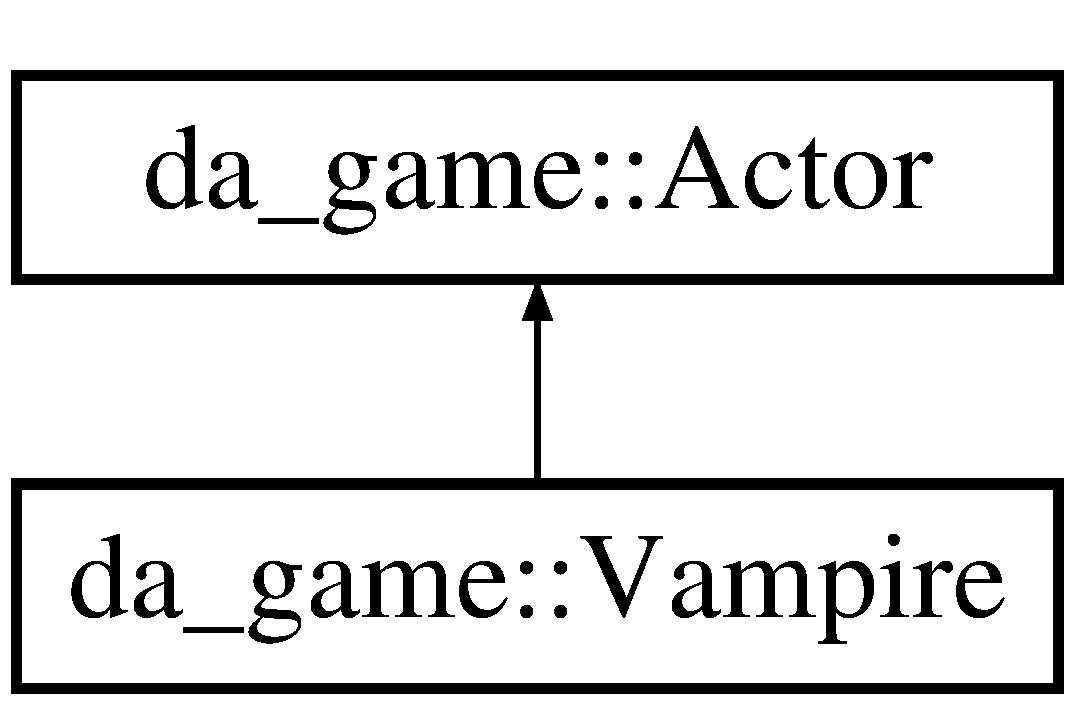
\includegraphics[height=2cm]{classda__game_1_1Vampire}
\end{center}
\end{figure}
\subsection*{Public Member Functions}
\begin{DoxyCompactItemize}
\item 
\hypertarget{classda__game_1_1Vampire_adfcf52e1ba7a0344f9d794c06a18da86}{
{\bfseries Vampire} (\hyperlink{classda__game_1_1Environment}{Environment} $\ast$, int, int)}
\label{classda__game_1_1Vampire_adfcf52e1ba7a0344f9d794c06a18da86}

\item 
\hypertarget{classda__game_1_1Vampire_a098285187dd2b419c4203fc871d41301}{
void {\bfseries eat} (\hyperlink{classda__game_1_1Actor}{Actor} \&)}
\label{classda__game_1_1Vampire_a098285187dd2b419c4203fc871d41301}

\item 
\hypertarget{classda__game_1_1Vampire_a67a45b375b34dcae9279f10a80c251cf}{
void {\bfseries eat} (\hyperlink{classda__game_1_1Food}{Food} \&)}
\label{classda__game_1_1Vampire_a67a45b375b34dcae9279f10a80c251cf}

\item 
\hypertarget{classda__game_1_1Vampire_aa026ac29df5be82f7305229780436621}{
virtual void {\bfseries run} ()}
\label{classda__game_1_1Vampire_aa026ac29df5be82f7305229780436621}

\item 
\hypertarget{classda__game_1_1Vampire_ae94c70e1a63a58ad3d5d77e4f0867200}{
virtual std::string {\bfseries get\_\-type} () const }
\label{classda__game_1_1Vampire_ae94c70e1a63a58ad3d5d77e4f0867200}

\item 
\hypertarget{classda__game_1_1Vampire_a461a139a2ba6c4f0714dc4824a132753}{
virtual std::string {\bfseries get\_\-name} () const }
\label{classda__game_1_1Vampire_a461a139a2ba6c4f0714dc4824a132753}

\item 
\hypertarget{classda__game_1_1Vampire_ab1826abb3ee4542d631e49241dbbb4cb}{
virtual void {\bfseries fight} (\hyperlink{classda__game_1_1Actor}{Actor} \&)}
\label{classda__game_1_1Vampire_ab1826abb3ee4542d631e49241dbbb4cb}

\item 
\hypertarget{classda__game_1_1Vampire_a94c6fce61816fed384b08da30c76ff63}{
virtual void {\bfseries pick\_\-up} (\hyperlink{classda__game_1_1Object}{Object} $\ast$)}
\label{classda__game_1_1Vampire_a94c6fce61816fed384b08da30c76ff63}

\item 
\hypertarget{classda__game_1_1Vampire_a49dcdd308b3e5a6865b4eb46c5d9f0fb}{
virtual bool {\bfseries drop} (\hyperlink{classda__game_1_1Object}{Object} $\ast$)}
\label{classda__game_1_1Vampire_a49dcdd308b3e5a6865b4eb46c5d9f0fb}

\item 
\hypertarget{classda__game_1_1Vampire_ae435892f6850a3e3fab698e35203149c}{
virtual void {\bfseries talk\_\-to} (\hyperlink{classda__game_1_1Actor}{Actor} \&)}
\label{classda__game_1_1Vampire_ae435892f6850a3e3fab698e35203149c}

\end{DoxyCompactItemize}


The documentation for this class was generated from the following files:\begin{DoxyCompactItemize}
\item 
vampire.h\item 
vampire.cpp\end{DoxyCompactItemize}

\hypertarget{classda__game_1_1VampireFactory}{
\section{da\_\-game::VampireFactory Class Reference}
\label{classda__game_1_1VampireFactory}\index{da\_\-game::VampireFactory@{da\_\-game::VampireFactory}}
}
Inheritance diagram for da\_\-game::VampireFactory::\begin{figure}[H]
\begin{center}
\leavevmode
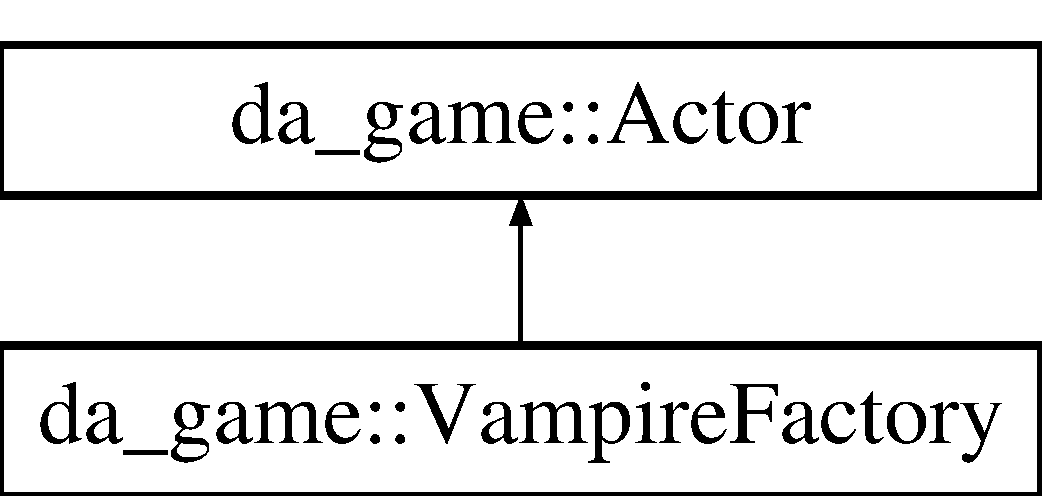
\includegraphics[height=2cm]{classda__game_1_1VampireFactory}
\end{center}
\end{figure}
\subsection*{Public Member Functions}
\begin{DoxyCompactItemize}
\item 
\hypertarget{classda__game_1_1VampireFactory_a9a3e0ab44708348be1caf55d7de920d5}{
{\bfseries VampireFactory} (\hyperlink{classda__game_1_1Environment}{Environment} $\ast$, int)}
\label{classda__game_1_1VampireFactory_a9a3e0ab44708348be1caf55d7de920d5}

\item 
\hypertarget{classda__game_1_1VampireFactory_a5981dc60b9f6fae2ce999e4555106d79}{
virtual void {\bfseries run} ()}
\label{classda__game_1_1VampireFactory_a5981dc60b9f6fae2ce999e4555106d79}

\item 
\hypertarget{classda__game_1_1VampireFactory_a9e156f9b668e710fb81cc4c0028cde17}{
virtual std::string {\bfseries get\_\-name} () const }
\label{classda__game_1_1VampireFactory_a9e156f9b668e710fb81cc4c0028cde17}

\item 
\hypertarget{classda__game_1_1VampireFactory_a4f48868efb55fb3b85c89738a0ab7c7d}{
virtual std::string {\bfseries get\_\-type} () const }
\label{classda__game_1_1VampireFactory_a4f48868efb55fb3b85c89738a0ab7c7d}

\item 
virtual void \hyperlink{classda__game_1_1VampireFactory_ab8f8fffebef4af1a90d00a0f011b245b}{go} (std::string)
\item 
\hypertarget{classda__game_1_1VampireFactory_a45b83b5acb2b73c475b9833119b9763b}{
virtual void {\bfseries fight} (\hyperlink{classda__game_1_1Actor}{Actor} \&)}
\label{classda__game_1_1VampireFactory_a45b83b5acb2b73c475b9833119b9763b}

\item 
\hypertarget{classda__game_1_1VampireFactory_a6cc92702b9e963c5e62340ec4036cd39}{
virtual void {\bfseries talk\_\-to} (\hyperlink{classda__game_1_1Actor}{Actor} \&)}
\label{classda__game_1_1VampireFactory_a6cc92702b9e963c5e62340ec4036cd39}

\end{DoxyCompactItemize}


\subsection{Member Function Documentation}
\hypertarget{classda__game_1_1VampireFactory_ab8f8fffebef4af1a90d00a0f011b245b}{
\index{da\_\-game::VampireFactory@{da\_\-game::VampireFactory}!go@{go}}
\index{go@{go}!da_game::VampireFactory@{da\_\-game::VampireFactory}}
\subsubsection[{go}]{\setlength{\rightskip}{0pt plus 5cm}void da\_\-game::VampireFactory::go (std::string {\em exit\_\-name})\hspace{0.3cm}{\ttfamily  \mbox{[}virtual\mbox{]}}}}
\label{classda__game_1_1VampireFactory_ab8f8fffebef4af1a90d00a0f011b245b}
Takes this actor to the environment that the given exit leads to. However the exit must not be locked.


\begin{DoxyParams}{Parameters}
\item[{\em exit\_\-name}]The name of the exit to go through \end{DoxyParams}


Reimplemented from \hyperlink{classda__game_1_1Actor_a6be7923ecbacabf779eda60f1f78bb72}{da\_\-game::Actor}.

The documentation for this class was generated from the following files:\begin{DoxyCompactItemize}
\item 
vampire\_\-factory.h\item 
vampire\_\-factory.cpp\end{DoxyCompactItemize}

\hypertarget{classda__game_1_1Wand}{
\section{da\_\-game::Wand Class Reference}
\label{classda__game_1_1Wand}\index{da\_\-game::Wand@{da\_\-game::Wand}}
}
Inheritance diagram for da\_\-game::Wand::\begin{figure}[H]
\begin{center}
\leavevmode
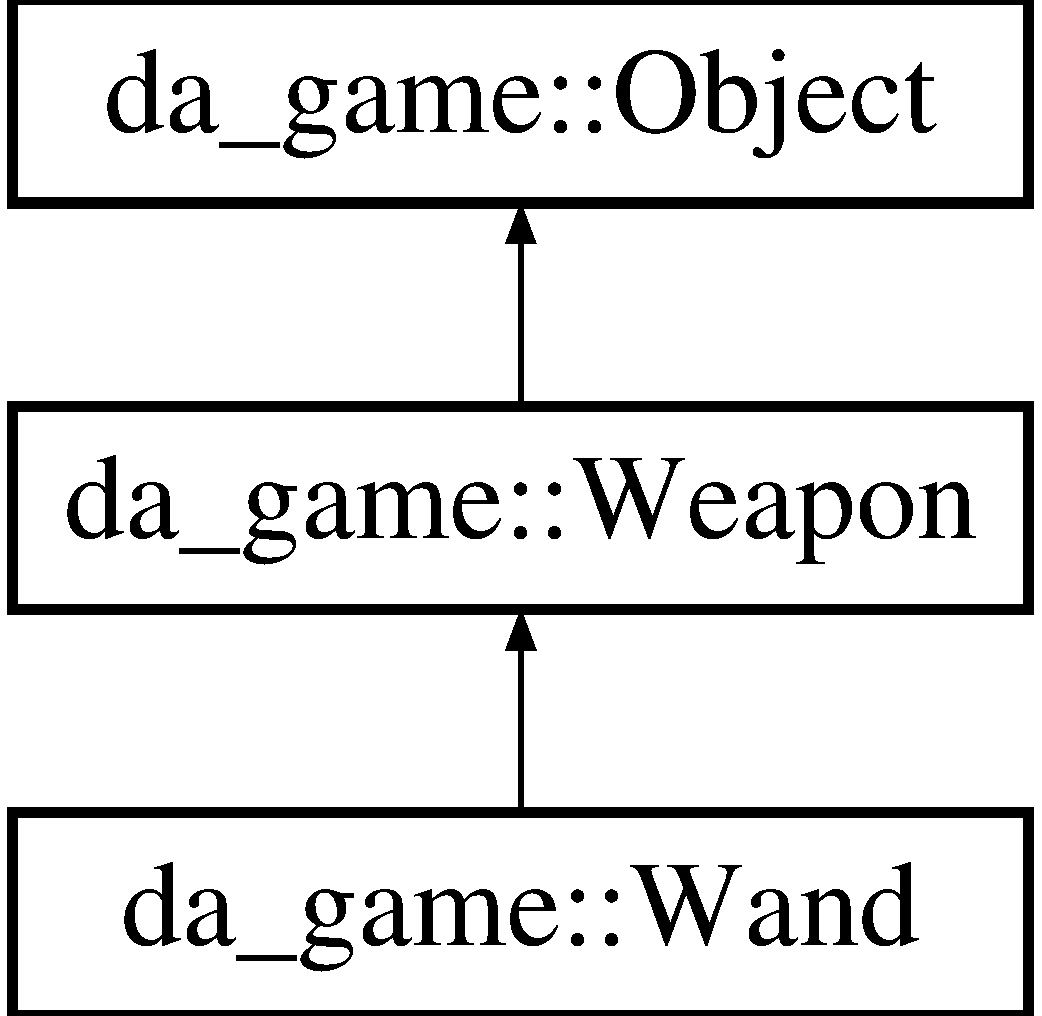
\includegraphics[height=3cm]{classda__game_1_1Wand}
\end{center}
\end{figure}
\subsection*{Public Member Functions}
\begin{DoxyCompactItemize}
\item 
\hypertarget{classda__game_1_1Wand_ae558206db7df170d40b3dfb32b1ce4cd}{
{\bfseries Wand} (unsigned int, float)}
\label{classda__game_1_1Wand_ae558206db7df170d40b3dfb32b1ce4cd}

\item 
\hypertarget{classda__game_1_1Wand_a20d019963c6c21c8b98c8cfd67e4edad}{
virtual int {\bfseries weight} () const }
\label{classda__game_1_1Wand_a20d019963c6c21c8b98c8cfd67e4edad}

\item 
\hypertarget{classda__game_1_1Wand_a85feab0eb776970c6b4ccd1d0bbd012f}{
virtual int {\bfseries volume} () const }
\label{classda__game_1_1Wand_a85feab0eb776970c6b4ccd1d0bbd012f}

\item 
\hypertarget{classda__game_1_1Wand_ac6d0ee9dddccc7b8b4a65ad1e137c2da}{
virtual int {\bfseries price} () const }
\label{classda__game_1_1Wand_ac6d0ee9dddccc7b8b4a65ad1e137c2da}

\item 
\hypertarget{classda__game_1_1Wand_ada77c13289de7d6a7ce00c39827c3023}{
virtual std::string {\bfseries type} () const }
\label{classda__game_1_1Wand_ada77c13289de7d6a7ce00c39827c3023}

\item 
\hypertarget{classda__game_1_1Wand_a9ae78043a8d08b22cb608b360f491ab3}{
virtual int {\bfseries magic\_\-cost} () const }
\label{classda__game_1_1Wand_a9ae78043a8d08b22cb608b360f491ab3}

\end{DoxyCompactItemize}


The documentation for this class was generated from the following files:\begin{DoxyCompactItemize}
\item 
wand.h\item 
wand.cpp\end{DoxyCompactItemize}

\hypertarget{classda__game_1_1Weapon}{
\section{da\_\-game::Weapon Class Reference}
\label{classda__game_1_1Weapon}\index{da\_\-game::Weapon@{da\_\-game::Weapon}}
}
Inheritance diagram for da\_\-game::Weapon::\begin{figure}[H]
\begin{center}
\leavevmode
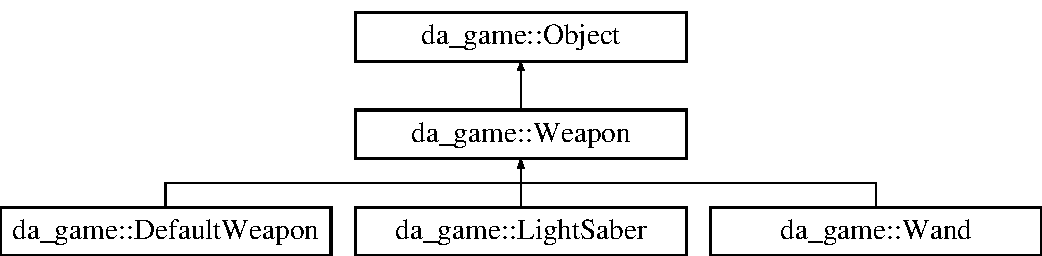
\includegraphics[height=3cm]{classda__game_1_1Weapon}
\end{center}
\end{figure}
\subsection*{Public Member Functions}
\begin{DoxyCompactItemize}
\item 
\hypertarget{classda__game_1_1Weapon_a88a5f2653bd77a5c4676871de3667604}{
{\bfseries Weapon} (unsigned int, float)}
\label{classda__game_1_1Weapon_a88a5f2653bd77a5c4676871de3667604}

\item 
\hypertarget{classda__game_1_1Weapon_a771944b2740e932845cec03eb644b563}{
virtual int {\bfseries weight} () const =0}
\label{classda__game_1_1Weapon_a771944b2740e932845cec03eb644b563}

\item 
\hypertarget{classda__game_1_1Weapon_a8769a66179398eb6b1b26b418c5cdb9f}{
virtual int {\bfseries volume} () const =0}
\label{classda__game_1_1Weapon_a8769a66179398eb6b1b26b418c5cdb9f}

\item 
\hypertarget{classda__game_1_1Weapon_aae5de95ab6a421f4799fc2f56fe04711}{
virtual int {\bfseries price} () const =0}
\label{classda__game_1_1Weapon_aae5de95ab6a421f4799fc2f56fe04711}

\item 
\hypertarget{classda__game_1_1Weapon_a0b5b2840ddee8fb059dd03849b2d4617}{
virtual std::string {\bfseries type} () const }
\label{classda__game_1_1Weapon_a0b5b2840ddee8fb059dd03849b2d4617}

\item 
\hypertarget{classda__game_1_1Weapon_ad0d737c1f1535fba0e1152daaa844a55}{
virtual int {\bfseries attack\_\-strength} () const }
\label{classda__game_1_1Weapon_ad0d737c1f1535fba0e1152daaa844a55}

\item 
\hypertarget{classda__game_1_1Weapon_a7ef8c157cc461a7fc1958f76652b0415}{
virtual float {\bfseries hit\_\-ratio} () const }
\label{classda__game_1_1Weapon_a7ef8c157cc461a7fc1958f76652b0415}

\end{DoxyCompactItemize}
\subsection*{Protected Attributes}
\begin{DoxyCompactItemize}
\item 
\hypertarget{classda__game_1_1Weapon_ac616cc0adf463730be8f90175b958309}{
unsigned int {\bfseries strength}}
\label{classda__game_1_1Weapon_ac616cc0adf463730be8f90175b958309}

\item 
\hypertarget{classda__game_1_1Weapon_ad712d94d84353fdae7dc4c0a82b52d91}{
float {\bfseries ratio}}
\label{classda__game_1_1Weapon_ad712d94d84353fdae7dc4c0a82b52d91}

\end{DoxyCompactItemize}


The documentation for this class was generated from the following files:\begin{DoxyCompactItemize}
\item 
weapon.h\item 
weapon.cpp\end{DoxyCompactItemize}

\hypertarget{classda__game_1_1Wizard}{
\section{da\_\-game::Wizard Class Reference}
\label{classda__game_1_1Wizard}\index{da\_\-game::Wizard@{da\_\-game::Wizard}}
}
Inheritance diagram for da\_\-game::Wizard::\begin{figure}[H]
\begin{center}
\leavevmode
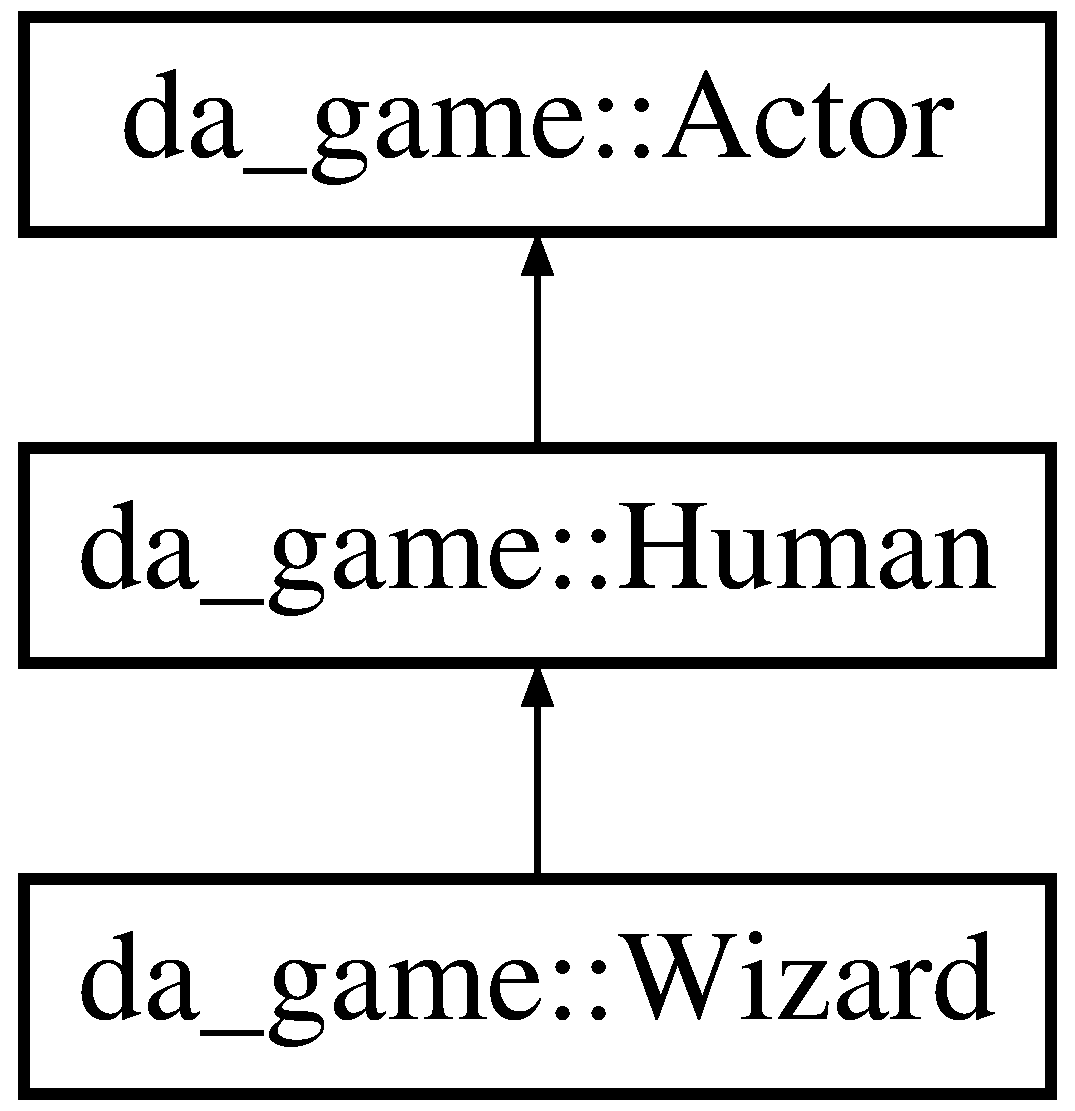
\includegraphics[height=3cm]{classda__game_1_1Wizard}
\end{center}
\end{figure}
\subsection*{Public Member Functions}
\begin{DoxyCompactItemize}
\item 
\hypertarget{classda__game_1_1Wizard_a12946b6b8b4377d3bc921f4acec267af}{
{\bfseries Wizard} (\hyperlink{classda__game_1_1Environment}{Environment} $\ast$, bool, int, int)}
\label{classda__game_1_1Wizard_a12946b6b8b4377d3bc921f4acec267af}

\item 
\hypertarget{classda__game_1_1Wizard_aea51ce7fcb9f92ca5176f5cbcbcb6775}{
virtual \hyperlink{classda__game_1_1Weapon}{Weapon} $\ast$ {\bfseries weapon} ()}
\label{classda__game_1_1Wizard_aea51ce7fcb9f92ca5176f5cbcbcb6775}

\item 
\hypertarget{classda__game_1_1Wizard_a774b9675e1817c6f7c2d0852a6c2f3bb}{
virtual std::string {\bfseries get\_\-name} () const }
\label{classda__game_1_1Wizard_a774b9675e1817c6f7c2d0852a6c2f3bb}

\item 
\hypertarget{classda__game_1_1Wizard_afd862632f5d1f6e2f0c0305226b3ebfd}{
virtual std::string {\bfseries get\_\-type} () const }
\label{classda__game_1_1Wizard_afd862632f5d1f6e2f0c0305226b3ebfd}

\item 
\hypertarget{classda__game_1_1Wizard_a242950311ea6d71faf9dfeb86918e510}{
virtual void {\bfseries run} ()}
\label{classda__game_1_1Wizard_a242950311ea6d71faf9dfeb86918e510}

\item 
\hypertarget{classda__game_1_1Wizard_aae7693d908c0e2d79bfc527cdb270548}{
virtual void {\bfseries talk\_\-to} (\hyperlink{classda__game_1_1Actor}{Actor} \&)}
\label{classda__game_1_1Wizard_aae7693d908c0e2d79bfc527cdb270548}

\end{DoxyCompactItemize}


The documentation for this class was generated from the following files:\begin{DoxyCompactItemize}
\item 
wizard.h\item 
wizard.cpp\end{DoxyCompactItemize}

\printindex
\end{document}
